\documentclass[12pt,a4paper,oneside]{report}
\usepackage{amsmath,amsthm}
\usepackage{fontspec}
\usepackage{unicode-math}
\setmainfont{TeX Gyre Termes}
\setsansfont{TeX Gyre Heros}
\setmonofont{DejaVu Sans Mono}[Scale=0.82]
\setmathfont{TeX Gyre Termes Math}
\usepackage{polyglossia}
\setdefaultlanguage{vietnamese}
\usepackage[left=3cm,right=2cm,top=2.5cm,bottom=2.5cm]{geometry}
\usepackage{graphicx,booktabs,longtable,array,tabularx,multirow,float,enumitem}
\usepackage{placeins}
\renewcommand{\topfraction}{0.9}\renewcommand{\bottomfraction}{0.8}
\renewcommand{\textfraction}{0.07}\renewcommand{\floatpagefraction}{0.75}
\setcounter{topnumber}{3}\setcounter{bottomnumber}{2}\setcounter{totalnumber}{5}
\usepackage[table]{xcolor}
\usepackage{adjustbox}
\usepackage{caption}
\captionsetup{font=small,labelfont=bf,labelsep=period}
\usepackage{titlesec,etoolbox}
\titleformat{\chapter}[display]{\normalfont\bfseries\Large\centering}{\MakeUppercase{\chaptername}~\thechapter}{6pt}{\LARGE}
\titlespacing*{\chapter}{0pt}{-10pt}{18pt}
\usepackage{fancyhdr}
\pagestyle{fancy}\fancyhf{}\fancyhead[R]{\small\nouppercase{\leftmark}}\fancyfoot[C]{\thepage}
\renewcommand{\headrulewidth}{0.3pt}
\setlength{\headheight}{15pt}
\usepackage[colorlinks=true,linkcolor=blue!40!black,citecolor=green!35!black,urlcolor=blue!40!black]{hyperref}
\linespread{1.25}
\setlength{\parskip}{4pt}
\theoremstyle{plain}
\newtheorem{menhde}{Mệnh đề}[chapter]
\theoremstyle{definition}
\newtheorem{dinhnghia}[menhde]{Định nghĩa}
\renewcommand{\proofname}{Chứng minh}
\newcommand{\R}{\mathbb{R}}
\newcommand{\E}{\mathbb{E}}
\setlist{itemsep=2pt,topsep=4pt}
\emergencystretch=1.5em
\setcounter{tocdepth}{1}
\makeatletter\patchcmd{\l@chapter}{1.0em}{0.15em}{}{}\makeatother
\newcommand{\TomTat}{Đồ án ước lượng trạng thái sức khoẻ (SOH) của cell lithium-ion từ 16 đặc trưng đoạn sạc khi chỉ một phần nhỏ cell được đo dung lượng, trên bốn bộ dữ liệu công khai (387 cell). Phân tích đặc trưng bằng tương quan hạng, bỏ từng nhóm đầu vào, độ quan trọng hoán vị và chọn trên tập xác thực cho thấy cả ba nhóm đặc trưng sạc và chỉ số chu kỳ đều mang thông tin. Chuẩn hoá theo cả vòng đời cell và lọc ngoại lai bằng tương lai của cell bị loại vì là rò rỉ. Kiểm toán cho thấy chia theo chu kỳ làm sai số thấp đi 1{,}2--1{,}8 lần và chuẩn hoá theo cả vòng đời cell làm sai số đổi 0{,}46--2{,}76 lần tuỳ bộ. Trong giao thức không rò rỉ (kiểm định chéo 5 fold theo cell, lặp lại, kiểm định ghép cặp), PINN bán giám sát có sai số bằng 0{,}39--0{,}90 lần MLP ở 10\,\% nhãn, nhưng GBDT vẫn tốt hơn nó khi có từ 30\,\% nhãn. Mô hình kết hợp PINN-lai, cấu hình chốt trước khi đọc tập kiểm tra, có sai số bằng 0{,}67--0{,}95 lần PINN-semi và thấp hơn GBDT ở 10/16 trường hợp. Trên đúng 39 nhóm đánh giá và với tiền xử lý của bài PINN4SOH, PINN-lai thấp hơn số công bố ở 11/12 chế độ và thấp hơn mã gốc của bài chạy lại ở 12/12, nhưng một GBDT cùng tiền xử lý đạt kết quả tương tự. Với tiền xử lý không rò rỉ, PINN-lai thấp hơn số công bố trên TJU và MIT, cao hơn trên HUST. Đo thưa mọi cell với 1{,}2--6{,}0\,\% số chu kỳ cho sai số bằng 0{,}85--0{,}93 lần gắn nhãn đầy đủ cho 30\,\% số cell. Đưa lịch sử của cell vào dự báo, đồ án xây dựng HiGBDT (GBDT có đặc trưng lịch sử SOH) và HiPINN, mô hình lấy trung vị của HiGBDT, PINN-dự báo và một nhánh theo đời cell. Khi có lịch sử đo dung lượng, HiPINN có sai số dự báo SOH bằng 0{,}62--0{,}91 lần PINN-GBDT, mô hình dự báo không có đặc trưng lịch sử.}

\begin{document}
\begin{titlepage}
\begin{center}
{\large ĐẠI HỌC QUỐC GIA THÀNH PHỐ HỒ CHÍ MINH\\[2pt]
\textbf{TRƯỜNG ĐẠI HỌC BÁCH KHOA}\\[2pt]
\textbf{KHOA KHOA HỌC VÀ KỸ THUẬT MÁY TÍNH}}\\[1.0cm]

\includegraphics[width=3.4cm]{hinh/bk.png}\\[1.2cm]
{\Large\textbf{ĐỒ ÁN CHUYÊN NGÀNH}}\\[1.4cm]
{\Large\bfseries DỰ ĐOÁN THÔNG SỐ SỨC KHOẺ CỦA PIN\\[4pt] BẰNG MÔ HÌNH HỌC SÂU ĐƯỢC HỖ TRỢ\\[4pt]
TỪ THÔNG TIN HOÁ LÝ CỦA HỆ PIN}\\[10pt]
{\large\itshape Health forecasting for battery systems using physics and chemistry-informed\\ deep learning methods}\\[1.6cm]
\end{center}
\begin{tabular}{@{\hspace{2.6cm}}ll}
Hướng đồ án: & Khoa học Máy tính\\[4pt]
Giảng viên hướng dẫn: & ......................................................\\[4pt]
Sinh viên thực hiện: & Huỳnh Quốc Thắng \quad MSSV: 2313178\\[4pt]
Nhóm: & 15\\[4pt]
Học kỳ: & HK261
\end{tabular}
\vfill
\begin{center}{\large TP. Hồ Chí Minh, tháng 11/2026}\end{center}
\end{titlepage}
\pagenumbering{roman}
\chapter*{Lời cam đoan}\addcontentsline{toc}{chapter}{Lời cam đoan}
Tôi xin cam đoan đồ án chuyên ngành ``Dự đoán thông số sức khoẻ của pin bằng mô hình học sâu được hỗ trợ từ thông
tin hoá lý của hệ pin'' là kết quả làm việc của riêng tôi dưới sự hướng dẫn của giảng viên hướng dẫn. Các bộ dữ liệu sử
dụng đều là dữ liệu công khai và được trích dẫn nguồn. Mọi số liệu, bảng và hình trong báo cáo được tính trực tiếp từ
kết quả thực nghiệm do tôi thực hiện; số liệu của các công trình khác được ghi rõ nguồn. Tôi xin chịu hoàn toàn trách
nhiệm nếu có bất kỳ sai phạm nào so với lời cam đoan này.

\vspace{1.2cm}
\hfill\begin{tabular}{c}TP. Hồ Chí Minh, tháng 11 năm 2026\\ Sinh viên thực hiện\\[1.6cm] Huỳnh Quốc Thắng\end{tabular}

\chapter*{Lời cảm ơn}\addcontentsline{toc}{chapter}{Lời cảm ơn}
Tôi xin chân thành cảm ơn giảng viên hướng dẫn đã định hướng đề tài, góp ý về phương pháp đánh giá và theo sát quá
trình thực hiện đồ án. Tôi cũng cảm ơn quý thầy cô Khoa Khoa học và Kỹ thuật Máy tính, Trường Đại học Bách khoa --
ĐHQG-HCM, đã trang bị nền tảng kiến thức để tôi thực hiện đề tài này. Cảm ơn các nhóm nghiên cứu tại Đại học Giao thông
Tây An, Đại học Thiên Tân, MIT--Stanford--Toyota Research Institute và Đại học Khoa học và Công nghệ Hoa Trung đã công bố
dữ liệu lão hoá pin, và nhóm tác giả PINN4SOH đã công bố mã nguồn cùng nhật ký huấn luyện, nhờ đó đồ án chạy lại được
kết quả của bài. Cuối cùng, tôi cảm ơn gia đình và bạn bè đã luôn động viên trong suốt thời gian thực hiện đồ án.

\chapter*{Tóm tắt}\addcontentsline{toc}{chapter}{Tóm tắt}
\TomTat

\noindent\textbf{Từ khoá:} pin lithium-ion, trạng thái sức khoẻ, PINN, học bán giám sát, chọn đặc trưng, rò rỉ dữ liệu,
kiểm định chéo, tái lập kết quả, PINN4SOH.
{\linespread{1.0}\selectfont\tableofcontents\listoffigures\listoftables}
\chapter*{Danh mục từ viết tắt}\addcontentsline{toc}{chapter}{Danh mục từ viết tắt}
\begin{center}\small
\begin{tabular}{>{\bfseries}l l}
\toprule
Viết tắt & Ý nghĩa \\
\midrule
BMS & Hệ thống quản lý pin (Battery Management System)\\
CC--CV & Sạc dòng không đổi -- áp không đổi (Constant Current -- Constant Voltage)\\
CNN & Mạng nơ-ron tích chập (Convolutional Neural Network)\\
GBDT & Cây quyết định tăng cường gradient (Gradient Boosting Decision Tree)\\
GPR & Hồi quy quá trình Gauss (Gaussian Process Regression)\\
KTC & Khoảng tin cậy\\
LAM & Mất vật liệu hoạt động (Loss of Active Material)\\
LFP & Lithium sắt phốt phát (LiFePO$_4$)\\
LLI & Mất lithium khả dụng (Loss of Lithium Inventory)\\
LSTM & Mạng bộ nhớ dài -- ngắn hạn (Long Short-Term Memory)\\
MAE & Sai số tuyệt đối trung bình (Mean Absolute Error)\\
MAPE & Sai số phần trăm tuyệt đối trung bình (Mean Absolute Percentage Error)\\
MLP & Perceptron nhiều lớp (Multilayer Perceptron)\\
NCA, NCM & Oxit niken--coban--nhôm, oxit niken--coban--mangan\\
PINN & Mạng nơ-ron có thông tin vật lý (Physics-Informed Neural Network)\\
PINN-semi & PINN bán giám sát, loss vật lý áp lên cả cell không nhãn\\
PINN-lai & Mô hình kết hợp: ba PINN-semi, GBDT và bộ lọc quỹ đạo\\
PINN4SOH & PINN của Wang và cộng sự (2024), bài gốc được chạy lại\\
RMSE & Căn bậc hai sai số bình phương trung bình (Root Mean Square Error)\\
RUL & Số chu kỳ còn lại tới ngưỡng cuối đời (Remaining Useful Life)\\
SEI & Lớp điện phân rắn trên bề mặt anode (Solid Electrolyte Interphase)\\
SOH & Trạng thái sức khoẻ (State of Health)\\
\bottomrule
\end{tabular}
\end{center}

\clearpage\pagenumbering{arabic}
\chapter*{Mở đầu}\addcontentsline{toc}{chapter}{Mở đầu}\markboth{Mở đầu}{}

Đồ án ước lượng trạng thái sức khoẻ (SOH) của cell lithium-ion từ dữ liệu đoạn sạc, trong điều kiện chỉ một phần nhỏ
các cell được đo dung lượng. Báo cáo gồm các nội dung: cơ sở lý thuyết (Chương~\ref{ch:lythuyet}); dữ liệu,
các đặc trưng được dùng và bị bỏ cùng số liệu chứng minh (Chương~\ref{ch:dactrung}); những việc đã thực hiện
(Chương~\ref{ch:thuchien}); kết quả chạy lại bài gốc PINN4SOH và các thí nghiệm của đồ án (Chương~\ref{ch:chaylai});
kết quả đạt được (Chương~\ref{ch:ketqua}); đối chiếu với các bài báo đã công bố, gồm cả các chỉ số tốt hơn và các chỉ
số chưa tốt (Chương~\ref{ch:sosanh}). Chương~\ref{ch:ketluan} tóm tắt những việc đã làm được và chưa làm được.

Mọi thí nghiệm dùng bốn bộ dữ liệu công khai XJTU, TJU, MIT và HUST (387 cell). Mọi con số trong bảng được sinh tự động
từ tệp kết quả của các lượt chạy; không số nào được gõ tay.

%% ============================================================================ CHƯƠNG 1
\chapter{Cơ sở lý thuyết}\label{ch:lythuyet}

Chương này trình bày các kiến thức mà đồ án dựa vào: bài toán ước lượng SOH, cơ chế suy giảm dung lượng, ý nghĩa của
đặc trưng đoạn sạc, các mô hình được so sánh, mạng nơ-ron có thông tin vật lý cùng mô hình PINN4SOH của bài gốc, học
bán giám sát, kết hợp mô hình, dự báo tuổi thọ còn lại, cách chọn đặc trưng và cách đánh giá mô hình khi dữ liệu có cấu
trúc nhóm.

\section{Trạng thái sức khoẻ và bài toán ước lượng}\label{sec:bai_toan}

Trong quá trình sử dụng, dung lượng của cell lithium-ion giảm dần. Trạng thái sức khoẻ đo mức suy giảm này bằng tỉ số
giữa dung lượng hiện tại và dung lượng danh định:
\begin{equation}
\mathrm{SOH}_n = \frac{Q_n}{Q_\text{danh định}},
\end{equation}
với $Q_n$ là dung lượng đo được ở chu kỳ thứ $n$. Hệ thống quản lý pin (BMS) cần SOH để ước tính quãng đường còn lại,
điều chỉnh chiến lược sạc và cảnh báo thời điểm thay pin; với pin xe điện, mốc cuối đời thường chọn ở SOH khoảng 0,8.

Muốn biết chính xác $Q_n$ phải xả đầy cell theo một quy trình chuẩn, mất nhiều giờ và phải dừng vận hành. Ngược lại,
điện áp và dòng điện lúc sạc được BMS ghi lại ở mọi chu kỳ của mọi cell. Bài toán vì vậy có dạng học ít nhãn: nhiều dữ
liệu đầu vào nhưng chỉ một phần nhỏ có nhãn.

Xét tập cell $\mathcal{C}$. Mỗi cell $c$ có chuỗi chu kỳ $n = 0, 1, \dots, L_c$; ở mỗi chu kỳ, từ đoạn sạc ta có vector
đặc trưng $\mathbf{x}_{c,n} \in \R^{16}$. Nhãn $y_{c,n} = \mathrm{SOH}_{c,n}$ chỉ được biết trên tập con các cell huấn
luyện $\mathcal{C}_L \subset \mathcal{C}_\text{train}$; các cell còn lại $\mathcal{C}_U = \mathcal{C}_\text{train}
\setminus \mathcal{C}_L$ chỉ có đặc trưng sạc. Mục tiêu là học hàm $\hat y = F(\mathbf{x}_{c,n}, n)$ sao cho sai số trên
các cell chưa từng xuất hiện khi huấn luyện là nhỏ nhất. Mô hình chỉ được dùng dữ liệu tới chu kỳ hiện tại, để chạy được
trực tuyến trong BMS. Bài toán thứ hai là dự báo: đứng ở chu kỳ $k$, dự báo SOH ở các chu kỳ $k + h$ và số chu kỳ còn lại
trước khi SOH xuống dưới ngưỡng cuối đời $\tau$ (RUL).

\section{Suy giảm dung lượng của pin lithium-ion}

Dung lượng của cell giảm theo hai nhóm cơ chế chính~\cite{birkl2017}: mất lithium khả dụng (LLI), chủ yếu do lớp SEI
phát triển trên bề mặt anode, và mất vật liệu hoạt động (LAM) do nứt hạt, bong tách hoặc hoà tan kim loại chuyển tiếp.
Giai đoạn đầu dung lượng thường giảm chậm và gần tuyến tính; về sau nhiều cell đi vào vùng ``đầu gối'', nơi tốc độ suy
giảm tăng nhanh~\cite{attia2022knee}. Các phản ứng phụ phụ thuộc nhiệt độ theo quy luật dạng Arrhenius: nhiệt độ cao làm
SEI phát triển nhanh hơn~\cite{waldmann2014}. Khi lớp SEI dày lên và bị giới hạn bởi khuếch tán, lượng lithium mất đi tỉ
lệ với căn bậc hai của thời gian~\cite{broussely2001,pinson2013}. Các mô hình thực nghiệm khớp mất mát dung lượng bằng
hàm luỹ thừa của điện lượng trao đổi nhân thừa số Arrhenius~\cite{wang2011lfp,schmalstieg2014}; chúng gọn nhưng cần bộ hệ
số riêng cho mỗi hệ hoá học và không mô tả được đoạn đầu gối~\cite{fermin2020}. Ba quan sát định tính được đồ án dùng làm
ràng buộc: dung lượng không tự tăng theo thời gian vận hành, suy giảm nhanh dần khi pin già, và nhanh hơn khi nhiệt độ cao.

\section{Đặc trưng của đoạn sạc CC--CV}\label{sec:lt_dactrung}

Các cell trong dữ liệu được sạc theo quy trình CC--CV: sạc dòng không đổi tới điện áp cắt trên, rồi giữ điện áp không
đổi cho tới khi dòng giảm xuống ngưỡng cắt. Khi cell già, dung lượng giảm và điện trở trong tăng~\cite{birkl2017}, nên
với cùng quy trình sạc, điện lượng, thời gian và hình dạng đường điện áp, dòng điện của từng pha thay đổi theo; chiều
thay đổi cụ thể phụ thuộc hệ hoá học và quy trình sạc (Mục~\ref{sec:dt_lienquan}). PINN4SOH~\cite{wang2024} tóm mỗi lần sạc thành 16 đặc trưng thống kê lấy trên
một cửa sổ điện áp của pha CC và một cửa sổ dòng điện của pha CV, cùng điện lượng và thời gian của hai pha
(Bảng~\ref{tab:features}). Các đặc trưng này tính được ở mọi chu kỳ chỉ từ dữ liệu BMS ghi lúc sạc. Nhãn SOH thì đến từ
lần xả đầy; vì vậy đặc trưng lấy từ lần xả không được dùng làm đầu vào của bài toán ước lượng (Mục~\ref{sec:dt_bo}).

\section{Các mô hình học có nhãn cho dữ liệu dạng bảng}\label{sec:lt_bang}

Mỗi chu kỳ sau khi trích đặc trưng là một hàng của một bảng: 16 cột đặc trưng, một cột thời gian và một cột nhãn.

\paragraph{Hồi quy Ridge.} Tìm $\mathbf{w}$ cực tiểu $\|\mathbf{y} - X\mathbf{w}\|^2 + \alpha\|\mathbf{w}\|^2$; số hạng
chuẩn hoá $L_2$ làm mô hình tuyến tính ổn định khi các cột tương quan mạnh với nhau.

\paragraph{Hồi quy quá trình Gauss (GPR).} Đặt tiên nghiệm $f \sim \mathcal{GP}(0, k)$ với nhân RBF cộng nhiễu trắng; dự
đoán là kỳ vọng hậu nghiệm, kèm phương sai~\cite{rasmussen2006}. Chi phí $O(n^3)$ theo số điểm huấn luyện nên chỉ dùng
được với vài nghìn điểm.

\paragraph{Cây quyết định tăng cường gradient (GBDT).} Mô hình là tổng $F_M(\mathbf{x}) = \sum_{m=1}^{M} \eta\, h_m(\mathbf{x})$
của các cây hồi quy nhỏ; cây thứ $m$ được khớp với gradient âm của hàm mất mát tại $F_{m-1}$, với sai số bình phương
chính là phần dư~\cite{friedman2001}. Dạng histogram chia giá trị mỗi cột thành các ngăn để tìm điểm cắt
nhanh~\cite{ke2017}. Trên dữ liệu bảng cỡ vừa, mô hình cây thường vượt mạng nơ-ron vì học tốt các hàm không trơn và ít
bị ảnh hưởng bởi cột không mang thông tin~\cite{grinsztajn2022}.

\section{Học sâu cho dữ liệu chuỗi thời gian}\label{sec:lt_chuoi}

Dữ liệu lão hoá là chuỗi thời gian theo hai trục: trong một chu kỳ (điện áp, dòng điện theo thời gian) và qua các chu kỳ
(các đại lượng tóm tắt trôi dần khi cell già). Đồ án làm việc trên trục chu kỳ: mô hình ước lượng SOH ở chu kỳ $n$ từ
đặc trưng của chu kỳ đó, hoặc của cửa sổ $L$ chu kỳ gần nhất $\mathbf{x}_{n-L+1}, \dots, \mathbf{x}_n$.

\paragraph{MLP.} Mạng truyền thẳng $\hat y = f_K \circ \dots \circ f_1(\mathbf{x}_n)$, $f_k(\mathbf{h}) = \sigma(W_k
\mathbf{h} + \mathbf{b}_k)$, chỉ nhìn một chu kỳ.

\paragraph{CNN.} Tích chập một chiều dọc trục chu kỳ, $h_n = \sigma\bigl(\sum_{j=0}^{k-1} W_j \mathbf{x}_{n - j\delta} +
\mathbf{b}\bigr)$ với kích thước $k$ và độ giãn $\delta$; khi bộ lọc chỉ nhìn các chu kỳ trước, đầu ra không dùng dữ liệu
tương lai~\cite{bai2018tcn}.

\paragraph{LSTM.} Mạng hồi quy giữ trạng thái nhớ $\mathbf{c}_n = \mathbf{f}_n \odot \mathbf{c}_{n-1} + \mathbf{i}_n
\odot \tanh(W_c[\mathbf{h}_{n-1}, \mathbf{x}_n] + \mathbf{b}_c)$, đầu ra $\mathbf{h}_n = \mathbf{o}_n \odot
\tanh(\mathbf{c}_n)$; các cổng quên, vào, ra có dạng $\sigma(W[\mathbf{h}_{n-1}, \mathbf{x}_n] + \mathbf{b})$ và cho phép
giữ thông tin qua nhiều bước~\cite{hochreiter1997}.

\paragraph{Transformer.} Tầng tự chú ý tính $\mathrm{softmax}(QK^\top / \sqrt{d})\,V$ trên mọi cặp vị trí trong cửa
sổ~\cite{vaswani2017}; vì phép tính này không phân biệt thứ tự, một mã hoá vị trí hình sin được cộng vào đầu vào.

\section{Mạng nơ-ron có thông tin vật lý}\label{sec:lt_pinn}

Xét phương trình $\mathcal{N}[u] = 0$ với nghiệm $u(\mathbf{z})$. PINN~\cite{raissi2019} xấp xỉ $u$ bằng mạng $u_\varphi$ và
cực tiểu
\begin{equation}
\mathcal{L}(\varphi) = \frac{1}{|D|}\sum_{(\mathbf{z}, y) \in D}\big(u_\varphi(\mathbf{z}) - y\big)^2
 + \lambda \frac{1}{|P|}\sum_{\mathbf{z} \in P}\big(\mathcal{N}[u_\varphi](\mathbf{z})\big)^2,
\end{equation}
trong đó $D$ là tập điểm có nhãn và $P$ là tập điểm collocation chỉ cần đầu vào~\cite{karniadakis2021}. Số hạng thứ hai là
tín hiệu học không cần nhãn. Với pin, phương trình suy giảm không được biết chính xác nên một phần của $\mathcal{N}$ phải
học từ dữ liệu: động học hộp đen học toàn bộ, động học xám giữ cấu trúc vật lý và chỉ học phần chưa biết. Huấn luyện PINN
khó hơn mạng thường: gradient của các số hạng có thể chênh nhau nhiều bậc~\cite{wang2021grad}, và ràng buộc mềm làm mặt
mất mát khó tối ưu khi hệ số của phương trình lớn~\cite{krishnapriyan2021}.

\section{Mô hình PINN4SOH của bài gốc}\label{sec:lt_pinn4soh}

PINN4SOH~\cite{wang2024} là công trình gần nhất với đồ án: cùng bốn bộ dữ liệu, cùng 16 đặc trưng. Theo mã nguồn công bố:
\begin{itemize}
\item Mạng nghiệm $u = F(\mathbf{x}, t)$ nhận 16 đặc trưng và chỉ số chu kỳ, gồm một mạng mã hoá 17--60--60--32 với hàm
      kích hoạt sin và một đầu ra 32--32--1.
\item Mạng động học $G$ nhận $(\mathbf{x}, t, u, u_\mathbf{x}, u_t)$, 35 đầu vào, ba lớp 60 nút; phần dư là
      $f = u_t - G$.
\item Mỗi mẫu huấn luyện là một cặp chu kỳ liền nhau $(1, 2)$ của cùng cell. Hàm mất mát
      $\mathcal{L} = \mathcal{L}_\text{data} + \alpha\,\mathcal{L}_\text{PDE} + \beta\,\mathcal{L}_\text{mono}$, với
      $\mathcal{L}_\text{data}$ là sai số bình phương trên hai chu kỳ, $\mathcal{L}_\text{PDE}$ là trung bình $f^2$, và
      $\mathcal{L}_\text{mono}$ phạt SOH tăng giữa hai chu kỳ.
\item Tiền xử lý: lọc ngoại lai $3\sigma$ theo trung bình và độ lệch chuẩn của cả vòng đời cell, trên mọi cột kể cả
      dung lượng và chỉ số chu kỳ; chuẩn hoá min--max về $[-1, 1]$ 16 đặc trưng và chỉ số chu kỳ theo cả vòng đời của
      từng cell, kể cả cell test. Validation là 20\,\% số hàng chọn ngẫu nhiên của các cell huấn luyện.
\item Đánh giá: XJTU và TJU học một mô hình cho mỗi nhóm điều kiện (batch), MIT và HUST một mô hình cho cả bộ với một tập
      cell test cố định; thêm thí nghiệm ít mẫu chỉ có $K = 1, \dots, 4$ cell có nhãn. Sai số là MAE từng cell test, lấy
      trung bình qua cell, qua 10 lần chạy và qua các nhóm.
\end{itemize}
Chương~\ref{ch:chaylai} cho thấy trong bản mã đã sinh ra số liệu công bố, $\mathcal{L}_\text{mono} = \sum
\operatorname{ReLU}(y_2 - y_1)$ chỉ phụ thuộc nhãn nên không có gradient; các bản sửa sau đó đổi thành
$\sum \operatorname{ReLU}(u_2 - u_1)$ rồi $\sum \operatorname{ReLU}\big((u_2 - u_1)(y_1 - y_2)\big)$.

\section{Học bán giám sát}

Học bán giám sát tận dụng dữ liệu không nhãn qua một giả định về cấu trúc của dữ liệu. Các họ phổ biến dựa trên chính dự
đoán của mô hình: gán nhãn giả~\cite{lee2013}, chưng cất tri thức~\cite{hinton2015}, Mean Teacher~\cite{tarvainen2017}.
Đồ án dùng giả định vật lý: quỹ đạo SOH của mọi cell, kể cả cell chưa đo dung lượng, phải thoả phương trình suy giảm,
không tăng theo thời gian và nằm trong miền giá trị hợp lý. Các ràng buộc này tính được chỉ từ đặc trưng sạc, nên mỗi cell
không nhãn đều đóng góp gradient. Nhãn giả chỉ tốt bằng mô hình sinh ra nó; ràng buộc vật lý không phụ thuộc mô hình,
nhưng chỉ cho biết dạng của quỹ đạo, không cho biết mức SOH.

\section{Kết hợp mô hình và khoảng dự đoán}

Trung bình dự đoán của nhiều mô hình là cách đơn giản nhất để giảm phương sai: bagging~\cite{breiman1996}, stacking~\cite{wolpert1992},
hay vài mạng giống nhau với khởi tạo khác nhau~\cite{lakshminarayanan2017}. Dự đoán phù hợp (conformal
prediction)~\cite{vovk2005,lei2018} cho khoảng dự đoán không cần giả định phân phối: trên một tập hiệu chỉnh tách riêng,
lấy phân vị phù hợp của phần dư làm nửa độ rộng khoảng; nếu mẫu hiệu chỉnh và mẫu mới hoán đổi được cho nhau, độ phủ ít
nhất bằng mức đặt ra~\cite{angelopoulos2023}. Quyết định thay pin cần biết độ tin cậy của dự đoán, không chỉ một con
số~\cite{thelen2024}.

\section{Dự báo suy giảm và tuổi thọ còn lại}

Các cách dự báo dung lượng và RUL chia làm ba nhóm~\cite{hu2020joule}: khớp một hàm thực nghiệm lên lịch sử của chính cell
rồi ngoại suy, có thể kèm bộ lọc Bayes~\cite{he2011}; học từ nhiều cell một ánh xạ từ lịch sử tới dung lượng tương lai
hay tới RUL~\cite{zhang2018lstm,severson2019}; và ghép hai nhóm trên, lấy dạng hàm từ cơ chế suy giảm còn tham số học từ
dữ liệu. Nhóm thứ nhất rất nhạy với nhiễu và độ dài lịch sử, nhất là trước điểm đầu gối~\cite{attia2022knee}. Đánh giá RUL
thường dùng thêm tỉ lệ dự báo rơi trong một dải sai số tương đối quanh RUL thật~\cite{saxena2008}.

\section{Chọn đặc trưng}\label{sec:lt_chon}

Chọn đặc trưng nhằm bỏ các cột không mang thông tin, trùng thông tin hoặc không dùng được lúc triển khai. Có ba nhóm
phương pháp~\cite{guyon2003}. Nhóm lọc đánh giá từng cột độc lập với mô hình, ví dụ hệ số tương quan hạng Spearman
$\rho$ giữa cột và nhãn; $\rho$ đo quan hệ đơn điệu, không đòi hỏi tuyến tính. Nhóm bao (wrapper) đánh giá cả tập cột
bằng sai số của mô hình trên dữ liệu không dùng để huấn luyện~\cite{kohavi1997}: bỏ hoặc thêm một nhóm cột, huấn luyện
lại và so sai số. Nhóm nhúng dùng thông tin bên trong mô hình. Độ quan trọng hoán vị~\cite{breiman2001rf} xáo trộn giá
trị một cột giữa các mẫu để cắt liên hệ của nó với nhãn, rồi đo sai số tăng bao nhiêu; khi các cột tương quan mạnh, hoán
vị từng cột đánh giá thấp tầm quan trọng của cả nhóm vì mô hình lấy được thông tin từ cột còn lại~\cite{strobl2008}, nên
cần hoán vị theo nhóm. Ngoài sức dự đoán, một đặc trưng chỉ được dùng nếu tính được tại thời điểm dự đoán: đặc trưng có
dùng thông tin tương lai của cell hay thông tin của nhãn là rò rỉ, dù làm sai số trông thấp hơn.

\section{Đánh giá mô hình, rò rỉ dữ liệu và kiểm định}\label{sec:lt_danhgia}

Kiểm định chéo là cách chuẩn để ước lượng sai số tổng quát~\cite{arlot2010}. Khi dữ liệu có cấu trúc nhóm, ở đây là các
chu kỳ của cùng một cell, việc chia phải theo nhóm; nếu không, các mẫu gần như trùng nhau nằm ở cả hai phía train và test.
Rò rỉ dữ liệu là một nguyên nhân phổ biến khiến kết quả học máy trong khoa học không tái lập được; các dạng thường gặp gồm
chia sai đơn vị, tiền xử lý dùng thống kê của tập test và chọn mô hình trên tập test~\cite{kapoor2023,varma2006}.

\paragraph{Chỉ số.} Với $y_i$ là SOH đo và $\hat y_i$ là SOH dự đoán:
\begin{gather}
\mathrm{MAE} = \tfrac{1}{N}\textstyle\sum|\hat y_i - y_i|, \quad
\mathrm{RMSE} = \sqrt{\tfrac{1}{N}\textstyle\sum(\hat y_i - y_i)^2}, \quad
\mathrm{MAPE} = \tfrac{100\,\%}{N}\textstyle\sum\big|\tfrac{\hat y_i - y_i}{y_i}\big|, \\
R^2 = 1 - \frac{\sum(\hat y_i - y_i)^2}{\sum(y_i - \bar y)^2}, \qquad
\mathrm{MAE}_\text{cell} = \frac{1}{|\mathcal{C}_\text{test}|}\sum_{c}\frac{1}{n_c}\sum_{n}|\hat y_{c,n} - y_{c,n}|.
\end{gather}
Chỉ số chính là $\mathrm{MAE}_\text{cell}$: mỗi cell có một phiếu, nên cell có tuổi thọ dài không lấn át kết quả. Đây
cũng là cách PINN4SOH tính sai số.

\paragraph{Kiểm định.} So hai mô hình trên cùng các cell test bằng kiểm định dấu--hạng Wilcoxon ghép
cặp~\cite{wilcoxon1945} trên hiệu sai số của từng cell; khi so trên nhiều bộ dữ liệu, $p$ được hiệu chỉnh bằng phương
pháp Holm~\cite{holm1979} để kiểm soát xác suất mắc ít nhất một sai lầm loại I. Khoảng tin cậy của tỉ số sai số dùng
bootstrap phân vị~\cite{efron1993}, lấy lại mẫu theo cell. Vì các tập train của các fold chồng lấp nhau, MAE của các fold
không độc lập; phép $t$ hiệu chỉnh của Nadeau và Bengio~\cite{nadeau2003,bouckaert2004} là kiểm định bảo thủ ở mức fold
dùng để kiểm tra thêm~\cite{dietterich1998}.

%% ============================================================================ CHƯƠNG 2
\chapter{Dữ liệu và đặc trưng đầu vào}\label{ch:dactrung}

Chương này mô tả bốn bộ dữ liệu và cách tiền xử lý, liệt kê các đặc trưng được dùng, rồi trình bày các phương pháp và số
liệu cho thấy vì sao dùng chúng và vì sao bỏ các đặc trưng hay cách biến đổi khác.

\section{Bốn bộ dữ liệu}\label{sec:data}

Cả bốn bộ là cell hình trụ 18650 được sạc--xả lặp lại trong phòng thí nghiệm tới khi dung lượng giảm sâu.
\begin{itemize}
\item XJTU, Đại học Giao thông Tây An, công bố cùng PINN4SOH~\cite{wang2024}: 55 cell NCM, danh định 2,0\,Ah, sáu chế độ
      thí nghiệm (sạc 2C, sạc 3C, xả ngẫu nhiên R2.5 và R3, bước ngẫu nhiên RW, mô phỏng quỹ đạo vệ tinh) ở nhiệt độ phòng.
\item TJU, Zhu và cộng sự~\cite{zhu2022}: 130 cell thuộc ba nhóm hoá học (NCA, NCM, NCM+NCA), thử ở 25, 35 và
      45\,\textdegree C với nhiều tốc độ sạc, tạo thành chín nhóm điều kiện.
\item MIT, Severson và cộng sự~\cite{severson2019}: cell LFP/graphite 1,1\,Ah, nhiều giao thức sạc nhanh, ba đợt thí
      nghiệm, buồng nhiệt 30\,\textdegree C.
\item HUST, Ma và cộng sự~\cite{ma2022}: 77 cell LFP/graphite 1,1\,Ah, cùng chế độ sạc nhanh và 77 chế độ xả nhiều bước
      khác nhau, 30\,\textdegree C.
\end{itemize}
Đặc trưng đoạn sạc của cả bốn bộ được trích theo cùng một quy trình và công bố kèm PINN4SOH, nên bốn bộ có chung không
gian đặc trưng. Bảng~\ref{tab:datastats} tóm tắt dữ liệu sau tiền xử lý.

\begin{table}[!htbp]\centering\footnotesize
\caption[Thống kê bốn bộ dữ liệu sau tiền xử lý]{Thống kê bốn bộ dữ liệu sau tiền xử lý. “Nhóm” là số chế độ thí nghiệm khác nhau dùng để phân tầng.}\label{tab:datastats}
\begin{adjustbox}{max width=\textwidth}\begin{tabular}{llrrrcccc}\toprule
Bộ & Hoá học & Cell & Chu kỳ & Nhóm & Tuổi thọ (min / trung vị / max) & SOH đầu & SOH cuối & $Q_\text{dđ}$ (Ah) \\\midrule
XJTU & NCM & 55 & 22.431 & 6 & 110 / 392 / 942 & 0{,}83--1{,}00 & 0{,}78--0{,}89 & 2,0 \\
TJU & NCA/NCM & 130 & 56.697 & 9 & 25 / 377 / 1.246 & 0{,}88--0{,}98 & 0{,}66--0{,}90 & 3,5 / 2,5 \\
MIT & LFP & 125 & 82.450 & 3 & 36 / 622 / 2.156 & 0{,}95--1{,}00 & 0{,}82--0{,}97 & 1,1 \\
HUST & LFP & 77 & 144.224 & 1 & 1.123 / 1.855 / 2.672 & 1{,}06--1{,}12 & 0{,}80--0{,}82 & 1,1 \\
\textbf{Tổng} &  & 387 & 305.802 &  &  &  &  &  \\
\bottomrule\end{tabular}\end{adjustbox}\end{table}


\section{Tiền xử lý}\label{sec:prep}

\paragraph{Nhãn.} $y_{c,n} = Q_{c,n}/Q_\text{danh định}$. Chu kỳ thiếu dung lượng được giữ lại với nhãn trống và chỉ
dùng cho loss vật lý.

\paragraph{Lọc ngoại lai nhân quả.} Chu kỳ $n$ bị loại nếu có đặc trưng không hữu hạn, hoặc có đặc trưng lệch xa so với
50 chu kỳ liền trước của chính cell. Với đặc trưng thứ $j$:
\begin{equation}
m_{n,j} = \operatorname{median}(x_{n-50..n-1,\,j}), \quad
s_{n,j} = \max\!\Big(\tfrac{\mathrm{IQR}(x_{n-50..n-1,\,j})}{1{,}349},\, 0{,}01\,|m_{n,j}|\Big), \quad
z_{n,j} = \frac{|x_{n,j} - m_{n,j}|}{s_{n,j}},
\end{equation}
chu kỳ bị loại nếu $\max_j z_{n,j} > 5$ (cần ít nhất 10 chu kỳ lịch sử). Ngưỡng 5 được chọn trước khi huấn luyện để tỉ lệ
chu kỳ bị loại (1,6\,\%) tương đương bộ lọc $3\sigma$ dùng cả vòng đời (2,2\,\%). Bộ lọc chỉ nhìn đặc trưng, không nhìn
dung lượng, và chỉ nhìn quá khứ của cell.

\paragraph{Chuẩn hoá.} Mỗi đặc trưng được chuẩn hoá z-score bằng trung bình và độ lệch chuẩn tính trên các cell huấn
luyện (có nhãn và không nhãn): $\tilde{\mathbf{x}} = (\mathbf{x} - \boldsymbol\mu)/(\boldsymbol\sigma + 10^{-6})$. Biến
thời gian là $t_n = n/1000$ với $n$ là chỉ số chu kỳ gốc; hằng số 1000 dùng chung cho mọi cell.

\section{Các đặc trưng được dùng}\label{sec:dt_dung}

Mọi mô hình ước lượng SOH của đồ án nhận cùng 17 đầu vào: 16 đặc trưng đoạn sạc ở Bảng~\ref{tab:features} và biến
thời gian $t$. Mô hình chuỗi nhận thêm các chu kỳ trước của chính cell. Nhiệt độ không là đầu vào của mạng nghiệm; ở PINN-semi nó chỉ đi
vào thừa số Arrhenius của động học suy giảm (Mục~\ref{sec:pinn}).

\begin{table}[!htbp]\centering\small
\caption[Các đặc trưng đầu vào]{Các đặc trưng đầu vào, chia thành bốn nhóm dùng cho phép thử bỏ nhóm ở
Mục~\ref{sec:dt_bonhom}.}\label{tab:features}
\begin{tabularx}{\textwidth}{>{\raggedright}p{3.0cm}>{\raggedright}p{5.4cm}>{\raggedright\arraybackslash}X}
\toprule
Nhóm & Đặc trưng & Ý nghĩa \\
\midrule
V: điện áp pha CC (6) & trung bình, độ lệch chuẩn, độ nhọn, độ lệch, độ dốc, entropy & hình dạng đường điện áp trong
cửa sổ điện áp của pha dòng không đổi \\
I: dòng điện pha CV (6) & trung bình, độ lệch chuẩn, độ nhọn, độ lệch, độ dốc, entropy & hình dạng đường dòng điện trong
cửa sổ dòng của pha áp không đổi \\
QT: điện lượng và thời gian (4) & điện lượng nạp và thời gian của pha CC; của pha CV & cell nhận được bao nhiêu điện
lượng và trong bao lâu ở mỗi pha \\
t: thời gian (1) & $t = n/1000$ & tuổi của cell tính bằng số chu kỳ \\
\bottomrule
\end{tabularx}
\end{table}

Có ba lý do chọn bộ đầu vào này trước khi xét số liệu. Thứ nhất, cả 17 đầu vào tính được ở mọi chu kỳ từ dữ liệu BMS ghi
lúc sạc và từ bộ đếm chu kỳ, không cần đo dung lượng. Thứ hai, bốn bộ có chung 16 đặc trưng, nên cùng một mô hình chạy
được trên cả bốn. Thứ ba, đây đúng là đầu vào của PINN4SOH, nên so sánh với bài gốc chỉ khác ở mô hình và cách đánh giá.
Bản dữ liệu đồ án dùng là bản đã trích đặc trưng công bố kèm PINN4SOH, chỉ chứa 16 đặc trưng này và dung lượng; các
đặc trưng cần đường cong đầy đủ (ví dụ đường cong dung lượng gia tăng $\mathrm{d}Q/\mathrm{d}V$, điện áp hồi phục sau
sạc) đòi hỏi tải và xử lý lại dữ liệu thô của từng bộ, đồ án chưa làm. Các mục sau kiểm tra bằng số liệu rằng mỗi nhóm đều mang thông tin, và rằng các đặc trưng hay
cách biến đổi khác đã thử đều không nên dùng.

\section{Phương pháp kiểm tra}\label{sec:dt_pp}

Bốn phép kiểm tra, cùng dữ liệu đã tiền xử lý ở Mục~\ref{sec:prep}:
\begin{enumerate}
\item \emph{Mức liên quan và trùng lặp} (phương pháp lọc, không cần mô hình). Với mỗi đặc trưng, tính hệ số Spearman
      $\rho$ giữa đặc trưng và SOH trong từng cell (trung vị qua các cell, cùng tỉ lệ cell có $|\rho| \ge 0{,}5$) và gộp
      mọi chu kỳ của bộ. Hai đặc trưng có $|\rho| \ge 0{,}95$ với nhau trên mọi chu kỳ của bộ được coi là gần như trùng
      thông tin.
\item \emph{Bỏ hoặc thêm nhóm} (phương pháp bao). Huấn luyện lại GBDT với từng tập đầu vào trên đúng các fold không rò
      rỉ của đồ án (5 fold theo cell, lần lặp 0--2, cùng tập cell có nhãn), ở hai mức nhãn 10 và 70\,\% số cell, rồi so MAE
      theo cell trên test với bộ đầy đủ bằng kiểm định Wilcoxon ghép cặp theo cell, hiệu chỉnh Holm qua bốn bộ. GBDT được
      dùng vì là mô hình đơn lẻ mạnh nhất của đồ án (Mục~\ref{sec:labels}) và đủ nhanh để huấn luyện lại hàng trăm lần;
      với bộ đầy đủ, nó trùng từng bit với GBDT của các thí nghiệm chính.
\item \emph{Độ quan trọng hoán vị} trên test của mô hình đầy đủ: hoán vị một đặc trưng, hoặc cả một nhóm, giữa các hàng
      test và đo tỉ số MAE theo cell sau và trước hoán vị.
\item \emph{Chọn đặc trưng trên validation}: trong mỗi fold, bỏ các đặc trưng mà hoán vị trên validation làm sai số tăng
      dưới 1\,\%, huấn luyện lại và đánh giá trên test. Đây là cách chọn đặc trưng tự động không chạm tới test.
\end{enumerate}
Các cách biến đổi đầu vào khác (chuẩn hoá theo cả vòng đời cell, đặc trưng tương đối, đặc trưng có lịch sử) được kiểm tra
bằng các thí nghiệm riêng nêu ở Mục~\ref{sec:dt_bo}.

\section{Mức liên quan và trùng lặp}\label{sec:dt_lienquan}

Bảng~\ref{tab:relevance} cho thấy trong từng cell, chỉ số chu kỳ gần như tỉ lệ nghịch với SOH ($\rho$ trung vị từ −1{,}00 đến −0{,}94), điều dễ hiểu vì SOH giảm dần theo thời gian. Nhiều đặc trưng sạc cũng biến thiên chặt theo SOH; số đặc trưng có $|\rho|$ trung vị từ 0,9 trở lên là 4 ở XJTU, 9 ở TJU, 5 ở MIT và 7 ở HUST. Nhưng đặc trưng mạnh nhất không giống nhau giữa các bộ: điện lượng pha CV ở XJTU, thời gian pha CV ở TJU, trung bình điện áp ở MIT và thời gian pha CC ở HUST. Có đặc trưng còn đổi chiều theo hệ hoá học: độ nhọn dòng điện tăng theo SOH ở hai bộ LFP ($\rho$ 0{,}77 và 0{,}87) nhưng giảm ở XJTU và TJU (−0{,}70 và −0{,}98). Không đặc trưng nào yếu ($|\rho| < 0{,}3$) ở cả bốn bộ, nên không có lý do bỏ một đặc trưng chỉ vì tương quan thấp.

Một số cặp đặc trưng gần như trùng nhau ($|\rho| \ge 0{,}95$ trên mọi chu kỳ của bộ): 13 cặp ở XJTU, 4 cặp ở TJU, 3 cặp ở MIT và 14 cặp ở HUST, nhưng chỉ có cặp độ nhọn dòng điện và độ bất đối xứng dòng điện trùng ở cả bốn bộ. Một cặp trùng ở bộ này lại mang hai thông tin khác nhau ở bộ khác, nên với một tập đầu vào chung không thể bỏ cột nào chỉ vì trùng lặp. Trùng lặp cũng làm phép hoán vị từng cột đánh giá thấp tầm quan trọng của mỗi cột trong cặp, vì vậy các phép thử dưới đây bỏ và hoán vị theo nhóm. Ngoài ra, tương quan đơn biến không cho biết một đặc trưng có giúp phân biệt các cell khi đi cùng các đặc trưng khác hay không, nên việc giữ hay bỏ phải được thử trực tiếp bằng mô hình.

\begin{table}[!htbp]\centering\small\setlength{\tabcolsep}{4pt}
\caption[Tương quan hạng giữa từng đầu vào và SOH]{Hệ số Spearman $\rho$ giữa từng đầu vào và SOH: trung vị qua các cell của $\rho$ tính trong từng cell (cột “trong cell”), và $\rho$ trên mọi chu kỳ của bộ (cột “gộp”). Dấu âm: đầu vào giảm khi SOH tăng.}\label{tab:relevance}
\begin{adjustbox}{max width=\textwidth}\begin{tabular}{lrrrrrrrr}\toprule
 & \multicolumn{2}{c}{XJTU} & \multicolumn{2}{c}{TJU} & \multicolumn{2}{c}{MIT} & \multicolumn{2}{c}{HUST} \\\cmidrule(lr){2-3}\cmidrule(lr){4-5}\cmidrule(lr){6-7}\cmidrule(lr){8-9}
Đầu vào & trong cell & gộp & trong cell & gộp & trong cell & gộp & trong cell & gộp \\\midrule
trung bình điện áp & 0{,}56 & 0{,}32 & 0{,}05 & 0{,}19 & −0{,}99 & −0{,}75 & −0{,}94 & −0{,}58 \\
độ lệch chuẩn điện áp & −0{,}51 & −0{,}54 & 0{,}24 & 0{,}27 & −0{,}25 & 0{,}11 & −0{,}91 & −0{,}58 \\
độ nhọn điện áp & 0{,}42 & 0{,}45 & −0{,}56 & −0{,}30 & 0{,}97 & 0{,}55 & 0{,}95 & 0{,}63 \\
độ bất đối xứng điện áp & −0{,}59 & −0{,}32 & 0{,}07 & 0{,}01 & 0{,}97 & 0{,}45 & 0{,}95 & 0{,}63 \\
độ dốc điện áp & −0{,}19 & −0{,}06 & −0{,}95 & −0{,}61 & 0{,}88 & 0{,}28 & 0{,}45 & 0{,}13 \\
entropy điện áp & −0{,}18 & −0{,}05 & 0{,}61 & 0{,}29 & 0{,}78 & 0{,}81 & 0{,}97 & 0{,}78 \\
\addlinespace[2pt]
trung bình dòng điện & 0{,}61 & 0{,}42 & 0{,}88 & 0{,}57 & −0{,}78 & −0{,}52 & −0{,}72 & −0{,}48 \\
độ lệch chuẩn dòng điện & 0{,}64 & 0{,}48 & 0{,}54 & 0{,}41 & −0{,}62 & −0{,}41 & −0{,}39 & −0{,}37 \\
độ nhọn dòng điện & −0{,}70 & −0{,}45 & −0{,}98 & −0{,}59 & 0{,}77 & 0{,}51 & 0{,}87 & 0{,}55 \\
độ bất đối xứng dòng điện & −0{,}63 & −0{,}43 & −0{,}98 & −0{,}59 & 0{,}78 & 0{,}52 & 0{,}87 & 0{,}53 \\
độ dốc dòng điện & −0{,}93 & −0{,}81 & −1{,}00 & −0{,}53 & −0{,}59 & −0{,}10 & 0{,}25 & 0{,}09 \\
entropy dòng điện & −0{,}93 & −0{,}82 & −1{,}00 & −0{,}55 & 0{,}37 & 0{,}35 & 0{,}60 & 0{,}26 \\
\addlinespace[2pt]
điện lượng pha CC & −0{,}10 & −0{,}11 & 0{,}95 & 0{,}57 & 0{,}98 & 0{,}89 & 0{,}97 & 0{,}84 \\
thời gian pha CC & −0{,}09 & −0{,}01 & 0{,}95 & 0{,}74 & 0{,}98 & 0{,}90 & 0{,}97 & 0{,}84 \\
điện lượng pha CV & −0{,}94 & −0{,}82 & −1{,}00 & −0{,}69 & 0{,}34 & 0{,}30 & 0{,}55 & 0{,}24 \\
thời gian pha CV & −0{,}94 & −0{,}82 & −1{,}00 & −0{,}65 & 0{,}59 & 0{,}41 & 0{,}64 & 0{,}30 \\
\addlinespace[2pt]
$t$ (chỉ số chu kỳ) & −0{,}94 & −0{,}74 & −1{,}00 & −0{,}93 & −1{,}00 & −0{,}72 & −1{,}00 & −0{,}92 \\
\bottomrule\end{tabular}\end{adjustbox}\end{table}


\section{Bỏ hoặc thêm nhóm đặc trưng}\label{sec:dt_bonhom}

Bảng~\ref{tab:ablation} và Hình~\ref{fig:features} cho kết quả bỏ hoặc thêm nhóm ở 8 trường hợp (4 bộ $\times$ 2 mức nhãn), Bảng~\ref{tab:perm} cho độ quan trọng hoán vị của mô hình đủ 17 đầu vào.

\paragraph{Biến thời gian $t$.} Bỏ $t$ làm sai số tăng có ý nghĩa ở 6 trên 8 trường hợp, nhiều nhất 1{,}35 lần; trường hợp duy nhất có lợi là MIT 10\,\% (tỉ số 0{,}90). Ngược lại, chỉ dùng $t$ mà bỏ hết đặc trưng sạc cho sai số gấp 1{,}20--12{,}33 lần: tuổi của cell một mình không đủ để biết SOH, vì các cell già đi với tốc độ rất khác nhau (tuổi thọ trong mỗi bộ chênh nhau nhiều lần, Bảng~\ref{tab:datastats}). Hoán vị $t$ giữa các hàng test làm sai số tăng 1{,}47--8{,}10 lần, nên mô hình thật sự dùng biến này.

\paragraph{Ba nhóm đặc trưng sạc.} Không có trường hợp nào bỏ một nhóm mà sai số giảm có ý nghĩa. Nhóm V (điện áp pha CC) và nhóm QT (điện lượng, thời gian) mang nhiều thông tin nhất: bỏ nhóm V làm sai số tăng có ý nghĩa ở 6 trên 8 trường hợp, bỏ nhóm QT ở 4 trên 8, có trường hợp gần gấp đôi (1{,}99). Bỏ nhóm I (dòng điện pha CV) chỉ làm sai số tăng có ý nghĩa ở 2 trường hợp. Chỉ giữ nhóm QT và $t$, tức 5 đầu vào, kém bộ đầy đủ có ý nghĩa ở 6 trên 8 trường hợp. Phép hoán vị cho cùng nhận xét: hoán vị nhóm QT làm sai số tăng tới 18{,}82 lần, nhóm V tới 5{,}02 lần, nhóm I chỉ tới 3{,}00 lần.

\paragraph{Chọn đặc trưng tự động.} Khi bỏ các đầu vào mà hoán vị trên validation làm sai số tăng dưới 1\,\%, mỗi fold giữ lại trung vị 7--17 trên 17 đầu vào tuỳ bộ và mức nhãn; hay bị bỏ nhất là trung bình dòng điện, độ lệch chuẩn dòng điện và độ lệch chuẩn điện áp. Trên test, cách chọn này cho sai số bằng 0{,}99--1{,}02 lần bộ đầy đủ, không khác có ý nghĩa ở trường hợp nào, tức bớt đầu vào không làm mô hình tốt lên.

\paragraph{Đọc kết quả.} Mọi tập rút gọn đều kém bộ đầy đủ ở ít nhất một trường hợp, và các trường hợp có lợi (bỏ $t$ ở MIT 10\,\%; thêm 16 đặc trưng tương đối ở TJU 70\,\%) không lặp lại ở bộ khác. Chọn đầu vào riêng cho từng bộ dựa trên những kết quả này là chọn mô hình trên tập test, còn chọn riêng cho từng fold bằng validation thì không cải thiện. Vì vậy đồ án dùng chung bộ 17 đầu vào cho mọi bộ dữ liệu và mọi mô hình.

\begin{table}[!htbp]\centering\small\setlength{\tabcolsep}{4pt}
\caption[Bỏ hoặc thêm nhóm đầu vào với GBDT]{Bỏ hoặc thêm nhóm đầu vào, GBDT trên đúng các fold không rò rỉ (3 lần lặp $\times$ 5 fold). Hàng đầu: MAE theo cell ($\times10^{-3}$) với đủ 17 đầu vào. Các hàng sau: tỉ số MAE so với đủ 17 đầu vào. $^{*}$/$^{\dagger}$: thấp hơn/cao hơn có ý nghĩa (Wilcoxon ghép cặp theo cell, Holm qua bốn bộ).}\label{tab:ablation}
\begin{adjustbox}{max width=\textwidth}\begin{tabular}{lrrrrrrrr}\toprule
 & \multicolumn{2}{c}{XJTU} & \multicolumn{2}{c}{TJU} & \multicolumn{2}{c}{MIT} & \multicolumn{2}{c}{HUST} \\\cmidrule(lr){2-3}\cmidrule(lr){4-5}\cmidrule(lr){6-7}\cmidrule(lr){8-9}
Tập đầu vào & 10\,\% & 70\,\% & 10\,\% & 70\,\% & 10\,\% & 70\,\% & 10\,\% & 70\,\% \\\midrule
đủ 17 đầu vào (MAE) & 14{,}01 & 9{,}64 & 12{,}60 & 6{,}96 & 3{,}15 & 1{,}59 & 23{,}84 & 14{,}60 \\
\addlinespace[2pt]
bỏ $t$ & 1{,}12$^{\dagger}$ & 1{,}18$^{\dagger}$ & 1{,}32$^{\dagger}$ & 1{,}11$^{\dagger}$ & 0{,}90$^{*}$ & 1{,}01 & 1{,}30$^{\dagger}$ & 1{,}35$^{\dagger}$ \\
chỉ $t$ & 1{,}92$^{\dagger}$ & 2{,}67$^{\dagger}$ & 1{,}75$^{\dagger}$ & 3{,}03$^{\dagger}$ & 6{,}55$^{\dagger}$ & 12{,}33$^{\dagger}$ & 1{,}20$^{\dagger}$ & 1{,}86$^{\dagger}$ \\
bỏ nhóm V & 0{,}99 & 1{,}06$^{\dagger}$ & 1{,}03$^{\dagger}$ & 1{,}10$^{\dagger}$ & 1{,}02 & 1{,}16$^{\dagger}$ & 1{,}11$^{\dagger}$ & 1{,}32$^{\dagger}$ \\
bỏ nhóm I & 0{,}96 & 1{,}03 & 1{,}06$^{\dagger}$ & 1{,}05 & 1{,}00 & 1{,}00 & 1{,}01 & 1{,}06$^{\dagger}$ \\
bỏ nhóm QT & 1{,}05$^{\dagger}$ & 1{,}02$^{\dagger}$ & 1{,}00 & 1{,}00 & 1{,}73$^{\dagger}$ & 1{,}99$^{\dagger}$ & 1{,}01 & 1{,}02 \\
chỉ QT và $t$ & 0{,}96 & 1{,}12$^{\dagger}$ & 1{,}15$^{\dagger}$ & 1{,}33$^{\dagger}$ & 1{,}05 & 1{,}26$^{\dagger}$ & 1{,}17$^{\dagger}$ & 1{,}52$^{\dagger}$ \\
thêm 16 đặc trưng tương đối & 1{,}02 & 0{,}99 & 0{,}98 & 0{,}89$^{*}$ & 1{,}19$^{\dagger}$ & 1{,}14$^{\dagger}$ & 1{,}03 & 0{,}95 \\
chọn trên validation & 1{,}00 & 1{,}01 & 1{,}01 & 0{,}99 & 1{,}00 & 1{,}00 & 1{,}02 & 1{,}00 \\
thêm $1/T$ (chỉ TJU) & -- & -- & 0{,}99$^{*}$ & 1{,}00 & -- & -- & -- & -- \\
\bottomrule\end{tabular}\end{adjustbox}\end{table}

\begin{table}[!htbp]\centering\small\setlength{\tabcolsep}{4pt}
\caption[Độ quan trọng hoán vị trên test]{Độ quan trọng hoán vị trên test của GBDT đủ 17 đầu vào: tỉ số MAE theo cell khi hoán vị cả một nhóm (hoặc một đầu vào) giữa các hàng test so với khi không hoán vị, trung bình 15 fold. Bằng 1: mô hình không dùng thông tin của nhóm đó.}\label{tab:perm}
\begin{adjustbox}{max width=\textwidth}\begin{tabular}{lrrrrrrrr}\toprule
 & \multicolumn{2}{c}{XJTU} & \multicolumn{2}{c}{TJU} & \multicolumn{2}{c}{MIT} & \multicolumn{2}{c}{HUST} \\\cmidrule(lr){2-3}\cmidrule(lr){4-5}\cmidrule(lr){6-7}\cmidrule(lr){8-9}
Hoán vị & 10\,\% & 70\,\% & 10\,\% & 70\,\% & 10\,\% & 70\,\% & 10\,\% & 70\,\% \\\midrule
nhóm V (6) & 1{,}29 & 1{,}76 & 1{,}30 & 2{,}39 & 3{,}37 & 5{,}02 & 1{,}18 & 2{,}10 \\
nhóm I (6) & 1{,}32 & 1{,}77 & 1{,}83 & 3{,}00 & 1{,}14 & 1{,}70 & 1{,}12 & 1{,}68 \\
nhóm QT (4) & 2{,}16 & 2{,}59 & 1{,}30 & 1{,}98 & 8{,}41 & 18{,}82 & 1{,}40 & 1{,}93 \\
$t$ & 1{,}47 & 2{,}77 & 4{,}59 & 8{,}10 & 1{,}78 & 2{,}61 & 2{,}88 & 4{,}27 \\
\bottomrule\end{tabular}\end{adjustbox}\end{table}

\begin{figure}[!htbp]\centering
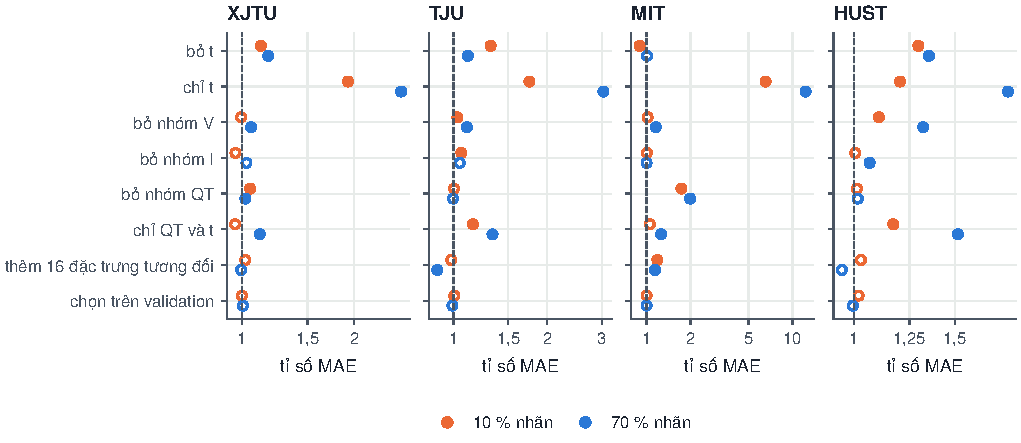
\includegraphics[width=\textwidth]{graphics/fig_features.pdf}
\caption[Bỏ hoặc thêm nhóm đầu vào: tỉ số MAE so với đủ 17 đầu vào]{Tỉ số MAE theo cell so với GBDT đủ 17 đầu vào, theo tập đầu vào và mức nhãn (thang log). Điểm đặc: khác có ý nghĩa (Wilcoxon theo cell, Holm qua bốn bộ); điểm rỗng: không có ý nghĩa. Vạch đứt: bằng bộ đầy đủ.}\label{fig:features}
\end{figure}


\section{Các đặc trưng và cách biến đổi đã bỏ}\label{sec:dt_bo}

Bảng~\ref{tab:dropped} tóm tắt những gì đã thử và bỏ. Ba dạng đầu là rò rỉ: chúng làm sai số đo được khác sai số thật khi triển khai, theo cả hai chiều tuỳ bộ (Bảng~\ref{tab:leak}), nên bị loại dù trên một số bộ chúng làm con số đẹp hơn. Đặc trưng tương đối bị loại ở bước chọn hướng cải tiến của PINN-lai vì làm sai số validation của PINN-semi tăng (tỉ số 1,692); phép chia cho mức ban đầu của cell khuếch đại các đặc trưng có giá trị ban đầu gần 0. Với GBDT, tác động của chúng trái chiều giữa các bộ (thấp hơn có ý nghĩa ở TJU 70\,\%, cao hơn có ý nghĩa ở MIT với cả hai mức nhãn), nên không dùng làm mặc định cho mọi bộ. Đặc trưng có lịch sử (Bảng~\ref{tab:hist} ở \Cref{sec:e20res}) giúp trên TJU và HUST khi có từ 30\,\% nhãn nhưng làm kém đi trên XJTU và ở 10\,\% nhãn, khi số chiều đầu vào tăng gấp đôi tới gấp bốn mà chỉ còn vài cell có nhãn; vì vậy PINN-lai không dùng chúng, còn HiPINN-lai chỉ dùng chúng ở các trường hợp validation chọn (\Cref{sec:pinnlai}, phân tích hậu kiểm). Nhiệt độ là hằng số trên ba bộ nên không mang thông tin; trên TJU, thêm $1/T$ vào GBDT cho tỉ số 0{,}99 (có ý nghĩa) ở 10\,\%, 1{,}00 ở 70\,\%, tức thay đổi dưới 1\,\%, nên nhiệt độ chỉ được giữ trong thừa số Arrhenius của động học. Đặc trưng từ lần xả và dung lượng các chu kỳ trước bị loại khỏi bài toán ước lượng vì đó chính là nhãn.

\begin{table}[!htbp]\centering\small
\caption[Các đặc trưng và cách biến đổi đã thử và bỏ]{Các đặc trưng và cách biến đổi đầu vào đã thử và bỏ, lý do và số liệu. Tỉ số là MAE so với cấu hình được dùng (lớn hơn 1: kém hơn; nhỏ hơn 1 ở hai hàng đầu: sai số trông thấp hơn thực tế vì rò rỉ).}\label{tab:dropped}
\begin{tabularx}{\textwidth}{>{\raggedright}p{3.6cm}>{\raggedright}p{4.2cm}>{\raggedright\arraybackslash}X}\toprule
Đã thử & Lý do bỏ & Số liệu \\\midrule
Chuẩn hoá min--max đặc trưng và $t$ theo cả vòng đời từng cell (như PINN4SOH) & dùng điểm cuối đời của cell, không có khi triển khai; $t$ sau chuẩn hoá là phần đời đã qua & MLP, 70\,\% nhãn: tỉ số XJTU 0{,}80, TJU 1{,}51, MIT 2{,}76, HUST 0{,}46 (Bảng~\ref{tab:leak}) \\
Lọc ngoại lai $3\sigma$ theo cả vòng đời, trên cả cột dung lượng & dùng tương lai của cell và cả nhãn & tỉ số 0{,}87--1{,}01 \\
Chuẩn hoá đặc trưng gồm cả cell test & dùng thống kê của tập test & tỉ số 0{,}98--1{,}03 \\
16 đặc trưng tương đối so với 3 chu kỳ đầu của cell & làm sai số validation của PINN-semi tăng; với GBDT tác động trái chiều giữa các bộ & PINN-semi, validation: tỉ số 1{,}692 (HUST 10\,\% nhãn: gấp 3{,}4 lần); GBDT, test: 0{,}89--1{,}19, cao hơn có ý nghĩa ở MIT với cả hai mức nhãn, thấp hơn có ý nghĩa ở TJU 70\,\% \\
Đặc trưng có lịch sử của cell (trung bình trượt mũ, độ dốc) & chỉ có lợi ở một số bộ khi đủ nhãn & Bảng~\ref{tab:hist}: PINN-lai 0{,}89--0{,}97 trên TJU, HUST từ 30\,\% nhãn; kém hơn trên XJTU (1{,}02--1{,}25); ở 10\,\% nhãn không giúp có ý nghĩa \\
Nhiệt độ làm đầu vào của mô hình & hằng số trên XJTU, MIT, HUST; trên TJU chỉ thay đổi sai số dưới 1\,\% & GBDT, TJU, thêm $1/T$: tỉ số 0{,}99$^{*}$ ở 10\,\%, 1{,}00 ở 70\,\% \\
Đặc trưng lấy từ lần xả, hoặc dung lượng đo của các chu kỳ trước & lần xả đầy chính là phép đo nhãn; khi ước lượng, dùng chúng là rò rỉ nhãn & chép nhãn chu kỳ gần nhất có sai số 0{,}01--0{,}15 lần mô hình thật (Bảng~\ref{tab:leak}); khi có đo thì dùng ở bước cập nhật (Mục~\ref{sec:budgetres}) \\
Đặc trưng cần đường cong thô (dung lượng gia tăng, điện áp hồi phục) & bản dữ liệu đã trích đặc trưng không có đường cong thô; chưa xử lý dữ liệu thô của từng bộ & chưa thử \\
\bottomrule\end{tabularx}\end{table}


\section{Kết luận về đầu vào}\label{sec:dt_ketluan}

Từ các kết quả trên, đồ án dùng đủ 16 đặc trưng đoạn sạc và $t = n/1000$: cả 17 tính được ở mọi chu kỳ từ dữ liệu sạc, 6 trên 6 tập rút gọn kém hơn có ý nghĩa ở ít nhất một trường hợp, không tập nào tốt hơn ở mọi bộ, và chọn bớt đặc trưng trên validation cho tỉ số 0{,}99--1{,}02. Đồ án không chuẩn hoá theo cả vòng đời cell, không lọc ngoại lai bằng tương lai của cell và không fit normaliser trên cell test, vì đây là rò rỉ và tác động của chúng lên sai số lên tới 0{,}46--2{,}76 lần tuỳ bộ. Đặc trưng tương đối không được dùng vì tác động trái chiều giữa các bộ; đặc trưng có lịch sử chỉ dùng khi validation chọn; nhiệt độ chỉ đi vào thừa số Arrhenius, vì thêm vào đầu vào chỉ thay đổi sai số dưới 1\,\%; thông tin của lần xả không được dùng khi ước lượng.


%% ============================================================================ CHƯƠNG 3
\chapter{Những việc đã thực hiện}\label{ch:thuchien}

Chương này mô tả những gì đồ án xây dựng: giao thức đánh giá không rò rỉ, mô hình PINN bán giám sát, mô hình kết hợp
PINN-lai, các mô hình đối chứng, quy trình chạy lại mã gốc PINN4SOH, các phần mở rộng và hệ thống mã nguồn.

\section{Giao thức đánh giá không rò rỉ}\label{sec:protocol}

\paragraph{Đơn vị chia là cell.} Các chu kỳ liên tiếp của một cell gần như giống nhau. Nếu chia ngẫu nhiên theo chu kỳ,
gần như mọi chu kỳ test đều có một chu kỳ kề bên trong train.

\begin{menhde}[Cận sai số khi chia theo chu kỳ]\label{md:rowleak}
Giả sử mỗi chu kỳ được đưa vào train độc lập với xác suất $q$. Xét bộ dự đoán không dùng đặc trưng nào, chỉ chép nhãn
của chu kỳ train gần nhất trong cùng cell. Bỏ qua hiệu ứng ở hai đầu cell, khoảng cách $d$ tới chu kỳ train gần nhất
thoả $\E[d] = 1/(1 - (1-q)^2)$, và sai số tuyệt đối kỳ vọng không vượt quá $\E[d]\cdot\overline{|\Delta y|}$, với
$\overline{|\Delta y|}$ là biến thiên nhãn trung bình giữa hai chu kỳ liền kề.
\end{menhde}
\begin{proof}
$d > j$ khi và chỉ khi $2j$ chu kỳ gần nhất về hai phía đều không thuộc train, xác suất $(1-q)^{2j}$, nên
$\E[d] = \sum_{j \ge 0} P(d > j) = 1/(1-(1-q)^2)$. Theo bất đẳng thức tam giác, sai số chép nhãn không vượt tổng $d$
biến thiên liền kề dọc quỹ đạo từ chu kỳ test tới chu kỳ train gần nhất; lấy kỳ vọng được
$\sum_{i \ge 0} P(d > i)\,\overline{|\Delta y|} = \E[d]\cdot\overline{|\Delta y|}$.
\end{proof}
Với $q = 0{,}7$, $\E[d] = 1{,}099$ chu kỳ: mô hình đánh giá theo cách chia này có thể đạt sai số rất thấp chỉ bằng cách
nhớ quỹ đạo. Đồ án chia theo cell: mọi chu kỳ của một cell nằm trọn trong train, validation hoặc test.

\paragraph{Fold, validation và lần lặp.} Kiểm định chéo 5 fold theo cell; mỗi fold dành 10\,\% số cell làm validation
(dừng sớm, chọn siêu tham số) và phần còn lại, 70\,\% số cell, làm train. Với 5 fold và 10\,\% validation, tập train vừa
đủ chứa mức nhãn cao nhất 70\,\% và bộ nhỏ nhất (XJTU) vẫn còn 11 cell test, 6 cell validation mỗi fold. Cách chia được
phân tầng theo chế độ thí nghiệm: trong mỗi chế độ, cell được xáo rồi chia vòng tròn với một bộ đếm chạy tiếp qua các chế
độ, nên mỗi cell được test đúng một lần ở mỗi lần lặp và số cell của một chế độ trong các fold lệch nhau không quá 1. Toàn
bộ lặp 5 lần với 5 cách xáo khác nhau (một số thí nghiệm về sau dùng 3 lần lặp đầu).

\paragraph{Mức nhãn.} 10, 30, 50 và 70\,\% số cell của bộ có nhãn, chọn từ các cell train theo một thứ tự vòng tròn cố
định qua các chế độ; tập có nhãn ở mức thấp là tập con của tập ở mức cao, nên khi tăng mức nhãn khác biệt duy nhất là có
thêm nhãn. Ở fold $k$ của lần lặp $r$, mọi mô hình dùng chung hạt giống $100r + k$: cùng cell train, cùng cell có nhãn,
cùng cell validation, cùng cell test, nên so được theo từng cell.

\paragraph{Bốn quy tắc chống rò rỉ.} (1) Normaliser chỉ fit trên đặc trưng của cell train. (2) Bộ lọc ngoại lai quyết
định giữ hay bỏ chu kỳ $n$ chỉ bằng các chu kỳ trước $n$ của chính cell. (3) Biến thời gian $t = n/1000$ dùng hằng số
chung. (4) Dừng sớm và chọn siêu tham số chỉ dựa trên validation; tập test chỉ dùng một lần để đánh giá.

\section{Mô hình PINN bán giám sát}\label{sec:pinn}

Mô hình gồm hai mạng nối với nhau qua hàm mất mát (Hình~\ref{fig:arch}). Mạng nghiệm $F_\varphi$ dự đoán SOH; mạng tốc
độ $G_\theta$ cùng hai tham số vật lý $\lambda, E_a$ mô tả tốc độ suy giảm. Khi suy luận chỉ cần $F_\varphi$.

\begin{figure}[!htbp]\centering
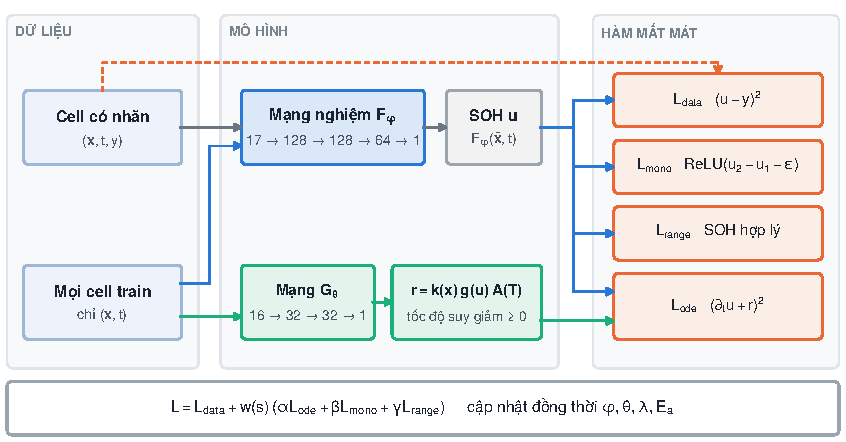
\includegraphics[width=\textwidth]{hinh/fig_arch.pdf}
\caption{Kiến trúc PINN bán giám sát: mạng nghiệm dự đoán SOH, mạng tốc độ mô tả động học suy giảm; hai mạng gắn với nhau
qua các hàm mất mát vật lý.}\label{fig:arch}
\end{figure}

\paragraph{Mạng nghiệm.} $u = F_\varphi(\tilde{\mathbf{x}}, t)$ là perceptron 17--128--128--64--1 với hàm kích hoạt SiLU.

\paragraph{Động học suy giảm dạng xám.}
\begin{equation}\label{eq:rate}
r(\tilde{\mathbf{x}}, u, T) =
\underbrace{\operatorname{softplus}\big(G_\theta(\tilde{\mathbf{x}})\big)}_{k(\mathbf{x})}\;
\underbrace{e^{\lambda\,\operatorname{clip}(1-u,\,-0{,}5,\,1)}}_{g(u)}\;
\underbrace{e^{-\frac{E_a}{R_g}\left(\frac{1}{T}-\frac{1}{T_\text{ref}}\right)}}_{A(T)},
\qquad \frac{\partial u}{\partial t} = -\,r(\tilde{\mathbf{x}}, u, T),
\end{equation}
với $G_\theta$ là perceptron 16--32--32--1, $\lambda = \operatorname{softplus}(\lambda_\text{raw})$,
$E_a = 10^4 \operatorname{softplus}(e_\text{raw})$\,J/mol, $T_\text{ref} = 298{,}15$\,K. Thừa số $k$ là tốc độ cơ sở
phụ thuộc trạng thái điện hoá (qua đặc trưng sạc), $g$ làm suy giảm tăng nhanh khi SOH thấp, $A$ là hệ số Arrhenius. Vì
softplus và hàm mũ đều dương, $r \ge 0$ với mọi tham số, nên mọi nghiệm của phương trình không tăng theo $t$.

\paragraph{Hàm mất mát.} Với cặp chu kỳ $(n_1, n_2)$ của cùng cell, $n_2 \ge n_1 + h$, $h \sim \mathcal{U}\{5, \dots,
50\}$, $u_i = F_\varphi(\tilde{\mathbf{x}}_{n_i}, t_{n_i})$:
\begin{align}
\mathcal{L}_\text{data} &= \tfrac{1}{B}\textstyle\sum (u - y)^2 && \text{(chỉ chu kỳ có nhãn)},\\
\mathcal{L}_\text{ode} &= \tfrac{1}{B}\textstyle\sum \big(\partial_t u_1 + r(\tilde{\mathbf{x}}_{n_1}, u_1, T)\big)^2, \\
\mathcal{L}_\text{mono} &= \tfrac{1}{B}\textstyle\sum \operatorname{ReLU}(u_2 - u_1 - \varepsilon), && \varepsilon = 0{,}002,\\
\mathcal{L}_\text{range} &= \tfrac{1}{B}\textstyle\sum \big[\operatorname{ReLU}(u_1 - 1{,}15) + \operatorname{ReLU}(0{,}4 - u_1)\big],
\end{align}
cộng một ràng buộc giữ SOH ở chu kỳ đầu của cell trong $[0{,}85;\,1{,}10]$;
\begin{equation}
\mathcal{L} = \mathcal{L}_\text{data} + w(s)\big(\alpha\mathcal{L}_\text{ode} + \beta\mathcal{L}_\text{mono}
+ \gamma\mathcal{L}_\text{range}\big), \qquad w(s) = \min\big(1, s/(0{,}2S)\big),
\end{equation}
với $\alpha = 0{,}02$, $\beta = 0{,}5$, $\gamma = 1$, $S = 4000$ bước; $\partial_t u$ tính bằng vi phân tự động.

\paragraph{Cơ chế bán giám sát.} Một nửa số cặp chu kỳ lấy từ cell có nhãn, một nửa từ cell không nhãn. Ba loss vật lý
không chứa $y$, chỉ phụ thuộc đặc trưng, thời điểm, nhiệt độ và tham số mô hình, nên tính được trên mọi cell chỉ có dữ
liệu sạc: mạng nghiệm bị buộc cho quỹ đạo hợp lý vật lý trên chính những cell mà nó phải tổng quát tới. Khác với
PINN4SOH, tốc độ $r$ không nhận $u_t$ làm đầu vào và luôn không âm, nên phần dư động học không thể được thoả mãn một cách
tầm thường bằng $G \approx u_t$.

\section{Mô hình kết hợp PINN-lai}\label{sec:pinnlai}

PINN-lai gồm ba bước:
\begin{align}
\bar F(\mathbf{x}, t) &= \tfrac{1}{3}\textstyle\sum_{m=1}^{3} F_{\varphi_m}(\tilde{\mathbf{x}}, t), \\
\hat y_n &= \tfrac{1}{2}\,\bar F(\mathbf{x}_n, t_n) + \tfrac{1}{2}\,g(\mathbf{x}_n, t_n), \\
\tilde y_n &= \bar y + \min(0, \hat\beta)\,(t_n - \bar t) \quad \text{trên cửa sổ } \hat y_{n-9}, \dots, \hat y_n,
\end{align}
với $F_{\varphi_m}$ là ba PINN-semi chỉ khác hạt giống, $g$ là GBDT học trên cùng các cell có nhãn, và bước cuối khớp một
đường thẳng có độ dốc không dương lên 10 dự đoán gần nhất của chính cell rồi lấy giá trị tại chu kỳ hiện tại (bộ lọc xu
thế nhân quả~\cite{cleveland1979}). Bộ lọc không làm lệch một quỹ đạo giảm tuyến tính, và với nhiễu độc lập phương sai
$\sigma^2$ nó giảm phương sai còn $0{,}345\,\sigma^2$ khi $w = 10$. Thành phần và trọng số được chọn trong 9 hướng cải tiến
chỉ bằng validation của lần lặp 0 (Mục~\ref{sec:e20res}); cấu hình được ấn định trước khi đọc dự đoán test.

\section{Mô hình đối chứng và cấu hình huấn luyện}\label{sec:baselines}

Mọi mô hình ở Bảng~\ref{tab:models} dùng cùng đầu vào, cùng cách chia, cùng tập cell có nhãn và cùng normaliser.

\begin{table}[!htbp]\centering\small
\caption{Các mô hình được so sánh.}\label{tab:models}
\begin{tabularx}{\textwidth}{l>{\raggedright}p{3.2cm}>{\raggedright\arraybackslash}X}
\toprule
Mô hình & Nhóm & Mô tả \\
\midrule
Ridge & học có nhãn & hồi quy tuyến tính chuẩn hoá $L_2$; $\alpha \in \{10^{-3},\dots,10^{3}\}$ chọn theo validation\\
GPR & học có nhãn & nhân RBF + nhiễu trắng, 1\,500 điểm có nhãn chọn ngẫu nhiên\\
GBDT & học có nhãn & dạng histogram, tốc độ học 0,05, 31 lá; số cây $\le 1000$ chọn theo validation\\
MLP & học có nhãn & cùng kiến trúc với mạng nghiệm, chỉ $\mathcal{L}_\text{data}$\\
CNN & học có nhãn, chuỗi & tích chập nhân quả, 32 kênh, kích thước 5, độ giãn 1 và 2, cửa sổ 16 chu kỳ\\
LSTM & học có nhãn, chuỗi & một lớp 32 nút ẩn, cửa sổ 48 chu kỳ\\
Transformer & học có nhãn, chuỗi & một lớp mã hoá 32 chiều, 4 đầu chú ý, mã hoá vị trí hình sin, cửa sổ 16 chu kỳ\\
PINN-sup & vật lý trên cell có nhãn & như PINN-semi nhưng loss vật lý chỉ tính trên cell có nhãn\\
PINN hộp đen & vật lý, bán giám sát & động học kiểu PINN4SOH, $u_t = G(\mathbf{x}, t, u, u_\mathbf{x}, u_t)$, cùng loss không nhãn\\
PINN-semi & vật lý, bán giám sát & mô hình đề xuất\\
PINN-lai & kết hợp & ba PINN-semi, GBDT, bộ lọc xu thế\\
\bottomrule
\end{tabularx}
\end{table}

MLP và các biến thể PINN dùng AdamW~\cite{loshchilov2019}, tốc độ học $2\cdot10^{-3}$ giảm theo cosine về $10^{-4}$ trong
4\,000 bước, batch 512 điểm có nhãn và 512 cặp chu kỳ, cắt gradient ở chuẩn 5, dừng sớm theo MAE validation. Độ dài cửa
sổ của CNN, LSTM và Transformer được chọn trong $\{16, 48\}$ trên validation. Trọng số vật lý được chọn trước ở một thí
nghiệm sơ bộ và giữ cố định; không siêu tham số nào được chọn theo tập test.

\section{Chạy lại mã gốc PINN4SOH}\label{sec:rerun_m}

Để so với bài gốc trên cùng điều kiện, đồ án chạy lại chính mã của bài:
\begin{enumerate}
\item \emph{Dựng lại cách chia.} Nhật ký huấn luyện công bố kèm mã ghi đường dẫn dữ liệu của từng lượt; từ đó dựng lại
      đúng 39 nhóm đánh giá: một nhóm cho mỗi batch của XJTU và TJU ở chế độ đầy đủ, một nhóm cho cả bộ MIT (23 cell test)
      và HUST (20 cell test), và các nhóm ít mẫu $K = 1, \dots, 4$ của XJTU và HUST.
\item \emph{Chạy nguyên trạng.} Lớp mô hình và lớp đọc dữ liệu của bài được dùng không sửa một dòng; đồ án chỉ viết phần
      gọi chúng, đặt hạt giống và ghi dự đoán theo từng cell test.
\item \emph{Hai bản mã.} Bản đã sinh ra số liệu công bố, với siêu tham số đọc từ nhật ký, chạy 10 lần mỗi nhóm như bài;
      bản hiện tại của kho mã (loss đơn điệu đã sửa, trọng số $\alpha, \beta$ mặc định mới), chạy 3 lần mỗi nhóm.
\item \emph{Đối chiếu nhật ký.} Nhật ký ghi giá trị loss đơn điệu ở mỗi epoch; đồ án tính lại biểu thức của loss này
      trên đúng các hàng train mà lớp đọc dữ liệu của bài tạo ra từ dữ liệu ở đây, rồi so với giá trị trong nhật ký.
\item \emph{Cùng điều kiện cho mô hình của đồ án.} PINN-lai, GBDT và PINN-semi được chạy trên đúng 39 nhóm đó với hai
      cách tiền xử lý: bản sao tiền xử lý của bài (có rò rỉ, chỉ để so cùng điều kiện) và tiền xử lý không rò rỉ của đồ
      án; mỗi nhóm 3 hạt giống.
\end{enumerate}
Mã gốc viết cho pandas 1.x; đồ án chạy nó trong một môi trường riêng có pandas 2.3, PyTorch 2 và trên CPU, trong khi bài
gốc dùng GPU và thư viện cũ hơn. Sai số được tính đúng như bài: MAE từng cell test, trung bình qua lần chạy, qua cell, qua
nhóm; so sánh ghép cặp theo cell bằng Wilcoxon, hiệu chỉnh Holm qua 12 tổ hợp bộ $\times$ chế độ.

\section{Ngân sách đo, cập nhật khi dùng và dự báo}\label{sec:mo_rong}

\paragraph{Nhãn thưa khi huấn luyện.} Thay vì đo đầy đủ một phần cell, mọi cell train được đo dung lượng ở chu kỳ đầu,
sau mỗi $qL$ chu kỳ ($L$ là trung vị số chu kỳ của cell train, $q \in \{0{,}5;\ 0{,}2;\ 0{,}1;\ 0{,}05\}$) và ở chu kỳ
cuối. PINN-semi chỉ tính $\mathcal{L}_\text{data}$ trên các chu kỳ được đo, còn loss vật lý vẫn tính trên mọi hàng; GBDT
học nhãn nội suy tuyến tính giữa các lần đo.

\paragraph{Cập nhật theo cell khi dùng.} Khi cell mới cũng được đo vài lần, sai số $y_n - p_n$ giữa SOH đo và SOH ước
lượng được mô hình hoá bằng một độ lệch trôi chậm hồi quy về trung bình (quá trình Ornstein--Uhlenbeck) cộng nhiễu, và
được cập nhật bằng bộ lọc Kalman mỗi khi có một lần đo; bốn tham số lấy trên validation. Một cách khác là mô hình cập
nhật: GBDT học thẳng SOH đã đổi bao nhiêu kể từ lần đo gần nhất.

\paragraph{Dự báo SOH, dung lượng và RUL.} Tại chu kỳ gốc $k$, một mạng nhỏ nhận tóm tắt lịch sử tới $k$ và trả hai tham
số $(a, \lambda)$ của nghiệm đóng của động học xám khi coi tốc độ cơ sở là hằng trong tầm dự báo:
\begin{equation}\label{eq:fcdrop}
\hat y(k+h) = \ell_k + \frac{1}{\lambda}\ln\bigl(1 - \lambda a h\bigr),
\end{equation}
với $\ell_k$ là mức SOH hiện tại; đường dự báo luôn không tăng và cong lên khi $\lambda > 0$ (đầu gối). Mô hình kết hợp
lấy trung bình với một GBDT học trực tiếp mức giảm theo tầm dự báo. RUL là tầm $h$ đầu tiên mà dự báo chạm ngưỡng
$\tau$. Lịch sử SOH tới gốc là dung lượng đo (khi có đo) hoặc ước lượng của PINN-lai (khi cell không được đo lần nào).

\section{Hiện thực và khối lượng tính toán}\label{sec:impl}

Hệ thống được hiện thực bằng Python thành một đường ống năm khối (Hình~\ref{fig:pipeline}), chạy được từ dữ liệu tới báo
cáo bằng một lệnh. Mỗi lượt huấn luyện là một tệp kết quả độc lập ghi đủ cấu hình, chỉ số, dự đoán validation và test;
bộ lập lịch chạy song song nhiều tiến trình một luồng, bỏ qua lượt đã có kết quả nên chạy tiếp được sau khi dừng. Khối
phân tích chỉ đọc các tệp kết quả, không huấn luyện lại. Báo cáo này và bản thảo bài báo được sinh từ kết quả phân tích,
nên mọi bảng đều khớp với dữ liệu. Mọi lượt chạy trên CPU với một luồng và hạt giống cố định, nên chạy lại cho kết quả
trùng từng bit (Chương~\ref{ch:chaylai}). Bảng~\ref{tab:exps} liệt kê các thí nghiệm.

\begin{figure}[!htbp]\centering
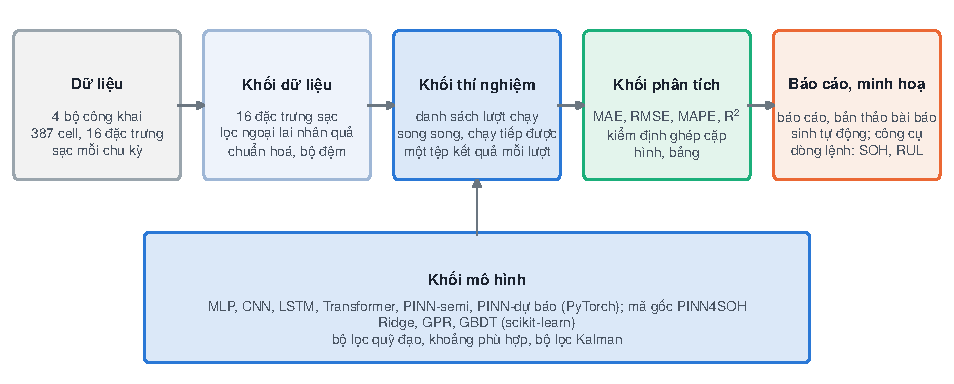
\includegraphics[width=\textwidth]{hinh/fig_pipeline.pdf}
\caption{Kiến trúc hiện thực: năm khối của hệ thống, từ dữ liệu tới báo cáo và công cụ minh hoạ.}\label{fig:pipeline}
\end{figure}

\begin{table}[!t]\centering\small
\caption[Các thí nghiệm có kết quả trong báo cáo]{Các thí nghiệm có kết quả trong báo cáo và số lượt huấn luyện (mỗi lượt là một mô hình trên một fold, hoặc một lần chạy trên một nhóm; lượt trùng cấu hình chỉ tính một lần).}\label{tab:exps}
\begin{tabularx}{\textwidth}{>{\raggedright\arraybackslash}X r}\toprule
Thí nghiệm & Lượt \\\midrule
Kiểm định chéo chính: MLP, PINN-semi ở 4 mức nhãn; PINN-sup và hai biến thể lược bỏ thành phần ở 30\,\% & 1.100 \\
Kiểm toán rò rỉ: 4 cách chia và chuẩn hoá sai, MLP 70\,\% nhãn & 160 \\
Ridge, GPR, GBDT ở 4 mức nhãn & 1.200 \\
PINN-sup ở 10 và 50\,\%; PINN hộp đen ở 4 mức nhãn & 600 \\
PINN-lai: 9 hướng cải tiến chọn trên tập xác thực; 3 PINN-semi, GBDT, 3 lần lặp, 4 mức nhãn & 1.680 \\
CNN, LSTM, Transformer: chọn độ dài cửa sổ trên tập xác thực; 3 lần lặp, 4 mức nhãn & 840 \\
Đầu vào có lịch sử của cell: chọn dạng trên tập xác thực; PINN-semi, MLP, GBDT & 1.190 \\
Ngân sách đo: đo thưa mọi cell huấn luyện theo 4 lịch đo & 1.560 \\
GBDT-cập nhật: cập nhật SOH từ lần đo gần nhất & 240 \\
Dự báo SOH, dung lượng, RUL: HiGBDT, HiPINN, các nhánh và mô hình đối chứng, 2 ngân sách nhãn, 3 lần lặp & 120 \\
HiGBDT cho bài toán cập nhật: GBDT-cập nhật, HiGBDT-$\Delta$, -R, -V trên 4 lịch đo & 60 \\
PINN-lai, GBDT và PINN-semi trên đúng 39 nhóm của PINN4SOH, 2 cách tiền xử lý, 3 hạt giống & 1.002 \\
Mã gốc PINN4SOH trên 39 nhóm đánh giá của bài, 10 lần mỗi nhóm & 390 \\
Phân tích đặc trưng: 120 fold $\times$ 9--10 lần huấn luyện GBDT với các tập đầu vào khác nhau & 1.110 \\
Độ nhạy của bộ lọc ngoại lai: GBDT với 7 cách đặt khác của bộ lọc, 4 bộ, 30\,\% nhãn & 420 \\
\midrule
Tổng & 11.672 \\
\bottomrule\end{tabularx}\end{table}


%% ============================================================================ CHƯƠNG 4
\chapter{Kết quả chạy lại}\label{ch:chaylai}

Chương này trình bày hai loại chạy lại: chạy lại mã gốc của PINN4SOH để có mốc so sánh đáng tin, và chạy lại các thí
nghiệm của chính đồ án để kiểm tra kết quả tái lập được.

\section{Chạy lại mã gốc PINN4SOH}\label{sec:rerun}

\paragraph{Cấu hình đã sinh ra số công bố.} Nhật ký huấn luyện ghi, ở mỗi epoch, giá trị trung bình của loss đơn điệu. Trong bản mã tải lên cùng bài báo, loss này là $\sum \operatorname{ReLU}(y_2 - y_1)$, chỉ tính từ nhãn của hai chu kỳ liền nhau. Ở cả 39 nhóm, giá trị ghi trong nhật ký là một hằng số qua mọi epoch của cả mười lần chạy, và ở cả 39 nhóm hằng số đó bằng đúng biểu thức trên tính trên các hàng train mà lớp đọc dữ liệu của bài tạo ra từ dữ liệu ở đây (ví dụ 0{,}043214 ở batch 2C của XJTU). Số hạng này vì vậy chỉ cộng thêm một hằng số và không có gradient: số liệu công bố đến từ mô hình chỉ học với loss dữ liệu và loss PDE. Sự trùng khớp này cũng cho thấy cách chia dựng lại và dữ liệu ở đây cho đúng các hàng train của mọi nhóm công bố. Hai bản sửa sau đó đổi số hạng thành $\sum \operatorname{ReLU}(u_2 - u_1)$ rồi $\sum \operatorname{ReLU}\big((u_2 - u_1)(y_1 - y_2)\big)$, và ghi chú mới nhất của kho mã cho biết trọng số $\alpha, \beta$ đã đổi sau khi sửa lỗi; trọng số mặc định trong các script hiện tại không còn khớp với nhật ký.

\paragraph{Chạy lại.} Bảng~\ref{tab:bench} và Hình~\ref{fig:bench} cho kết quả. Bản đã sinh số công bố, chạy 10 lần mỗi nhóm với siêu tham số trong nhật ký, cho sai số bằng 1{,}04--1{,}19 lần số công bố ở bốn bộ đầy đủ và 0{,}97--1{,}20 lần ở chế độ ít mẫu. So theo từng cell test, bản chạy lại cao hơn số công bố có ý nghĩa ở 2 trên 4 bộ đầy đủ. Độ lệch chuẩn giữa các lần chạy bằng 4--34\,\% giá trị trung bình, nên các lần chạy đơn lẻ chênh nhau cỡ khoảng cách trên. Các hàng train trùng khớp, nên phần chênh còn lại đến từ phần cứng, phiên bản thư viện và hạt giống; đồ án không dựng lại được môi trường gốc nên không biết yếu tố nào gây ra phần chênh có hệ thống. Vì vậy báo cáo nêu cả số công bố lẫn số chạy lại, và dùng số chạy lại cho kiểm định ghép cặp vì có dự đoán theo từng cell trong điều kiện đã biết. Bản hiện tại của mã (3 lần mỗi nhóm) cho sai số bằng 0{,}93--1{,}02 lần bản công bố ở bốn bộ đầy đủ và ở chế độ ít mẫu của HUST (không trường hợp nào trong 8 khác có ý nghĩa), nhưng 1{,}54--1{,}87 lần ở chế độ ít mẫu của XJTU với $K \ge 2$ (cao hơn có ý nghĩa ở 2 trên 3), nơi script hiện tại vẫn đặt $\beta = 10$ cho loss đơn điệu nay đã có tác dụng.

\begin{table}[!htbp]\centering\small\setlength{\tabcolsep}{4pt}
\caption[So với PINN4SOH trên đúng cách chia của bài]{MAE theo cell ($\times10^{-3}$) trên đúng các nhóm của PINN4SOH, trung bình qua cell test, lần chạy và nhóm như bài. Chạy lại: mã gốc ở bản đã sinh số công bố (siêu tham số theo nhật ký, 10 lần chạy mỗi nhóm) và ở bản hiện tại (loss đơn điệu đã sửa, trọng số mặc định mới, 3 lần chạy); $\pm$ là độ lệch chuẩn qua lần chạy. Mô hình của đồ án: 3 hạt giống. $K$: số cell có nhãn trong thí nghiệm ít mẫu. $^{*}$/$^{\dagger}$: PINN-lai với tiền xử lý của bài thấp hơn/cao hơn có ý nghĩa so với mã gốc chạy lại bản công bố (Wilcoxon theo cell test, Holm qua 12 hàng).}\label{tab:bench}
\begin{adjustbox}{max width=\textwidth}\begin{tabular}{llrrrrrr}\toprule
 & & \multicolumn{3}{c}{PINN4SOH} & \multicolumn{2}{c}{tiền xử lý của bài} & không rò rỉ \\\cmidrule(lr){3-5}\cmidrule(lr){6-7}\cmidrule(lr){8-8}
Bộ & Chế độ & công bố & chạy lại, bản công bố & chạy lại, bản đã sửa & PINN-lai & GBDT & PINN-lai \\\midrule
XJTU & đầy đủ & 7{,}85 & 8{,}66 $\pm$ 1{,}04 & 8{,}08 $\pm$ 0{,}26 & 6{,}62 & 6{,}82 & 7{,}81 \\
TJU & đầy đủ & 9{,}79 & 11{,}21 $\pm$ 0{,}47 & 10{,}87 $\pm$ 0{,}22 & 8{,}78$^{*}$ & 8{,}63 & 6{,}16 \\
MIT & đầy đủ & 6{,}18 & 7{,}36 $\pm$ 0{,}69 & 7{,}48 $\pm$ 0{,}97 & 6{,}80 & 6{,}15 & 1{,}43 \\
HUST & đầy đủ & 7{,}57 & 7{,}90 $\pm$ 0{,}80 & 7{,}38 $\pm$ 0{,}37 & 6{,}45$^{*}$ & 6{,}16 & 12{,}51 \\
\addlinespace
XJTU & $K = 1$ & 31{,}54 & 30{,}70 $\pm$ 8{,}47 & 27{,}09 $\pm$ 8{,}35 & 10{,}51$^{*}$ & 10{,}20 & 13{,}27 \\
 & $K = 2$ & 10{,}06 & 11{,}54 $\pm$ 1{,}34 & 17{,}77 $\pm$ 0{,}99 & 7{,}72 & 8{,}22 & 13{,}60 \\
 & $K = 3$ & 7{,}98 & 9{,}24 $\pm$ 1{,}13 & 16{,}44 $\pm$ 0{,}27 & 7{,}15 & 7{,}04 & 9{,}48 \\
 & $K = 4$ & 7{,}62 & 9{,}17 $\pm$ 1{,}09 & 17{,}18 $\pm$ 0{,}53 & 7{,}20 & 7{,}04 & 8{,}39 \\
\addlinespace
HUST & $K = 1$ & 39{,}42 & 47{,}13 $\pm$ 15{,}83 & 48{,}28 $\pm$ 14{,}94 & 14{,}71$^{*}$ & 10{,}08 & 46{,}72 \\
 & $K = 2$ & 16{,}94 & 18{,}07 $\pm$ 3{,}15 & 16{,}77 $\pm$ 2{,}56 & 11{,}53$^{*}$ & 9{,}66 & 23{,}82 \\
 & $K = 3$ & 14{,}59 & 15{,}10 $\pm$ 1{,}41 & 14{,}68 $\pm$ 1{,}10 & 9{,}16$^{*}$ & 7{,}73 & 21{,}13 \\
 & $K = 4$ & 13{,}62 & 14{,}71 $\pm$ 0{,}60 & 14{,}48 $\pm$ 1{,}09 & 9{,}91$^{*}$ & 8{,}58 & 22{,}64 \\
\bottomrule\end{tabular}\end{adjustbox}\end{table}

\begin{figure}[!htbp]\centering
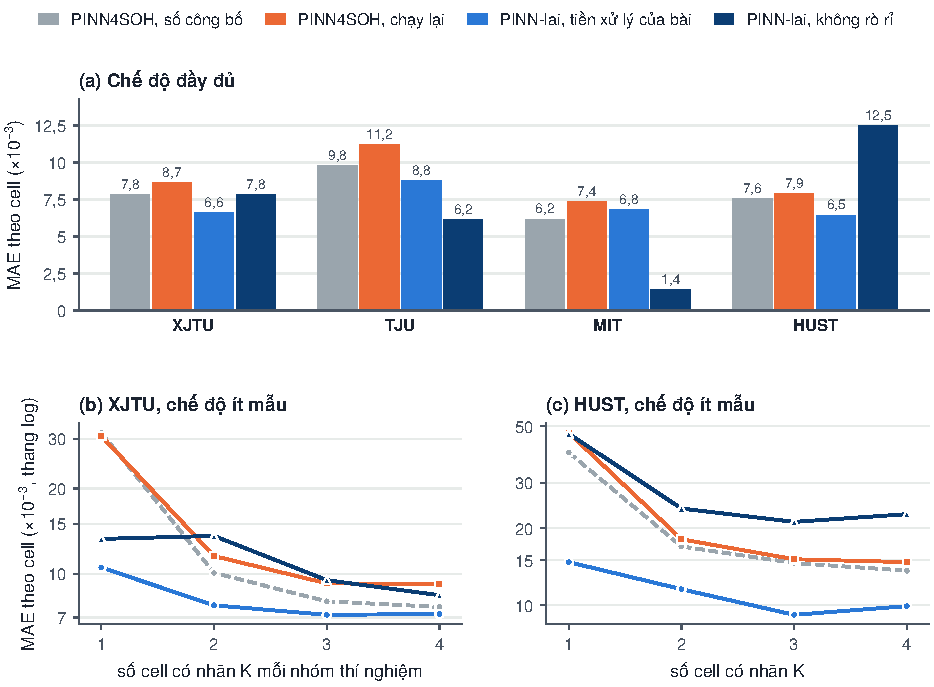
\includegraphics[width=\textwidth]{graphics/fig_benchmark.pdf}
\caption[So với PINN4SOH trên đúng cách chia của bài]{So với PINN4SOH trên đúng cách chia của bài. Trên: chế độ đầy đủ, mỗi bộ năm cột (số công bố, hai bản mã gốc chạy lại với độ lệch chuẩn qua lần chạy, PINN-lai với tiền xử lý của bài và với tiền xử lý không rò rỉ). Dưới: chế độ ít mẫu, MAE theo số cell có nhãn (thang log).}\label{fig:bench}
\end{figure}


\section{Chạy lại các thí nghiệm của đồ án}\label{sec:tailap}

Mọi lượt chạy dùng một luồng và hạt giống cố định, nên trên cùng loại CPU và cùng phiên bản thư viện, chạy lại phải cho dự đoán trùng từng bit. Các kiểm tra đã làm:

\begin{enumerate}
\item Hai mươi lượt mẫu phủ mọi loại thí nghiệm chính (MLP, PINN-semi, PINN-sup, PINN hộp đen, Ridge, GPR, GBDT, kiểm toán rò rỉ, chuyển miền), chạy lại vào thư mục tạm và so với giá trị lưu của lần chạy báo cáo đã nộp: 20 trên 20 lượt có MAE theo cell và mã băm của toàn bộ dự đoán test trùng từng bit.
\item Kiểm toán rò rỉ (160 lượt của bốn cách làm sai và 40 lượt tham chiếu theo cell) được chạy lại toàn bộ; 5 trên 5 lượt có giá trị tham chiếu lưu sẵn trùng từng bit, và các tỉ số ở Bảng~\ref{tab:leak} khớp với báo cáo đã nộp.
\item PINN-lai, GBDT và PINN-semi trên 39 nhóm của PINN4SOH (1.002 lượt) được chạy lại toàn bộ và so với kết quả của lần chạy trước: 216 trên 216 giá trị trung bình (MAE, RMSE và độ lệch chuẩn qua ba hạt giống của PINN-lai, GBDT và trung bình ba PINN-semi, với hai cách tiền xử lý, trên 12 chế độ) trùng từng bit; MAE và RMSE theo cell của cả 3.852 dòng trùng ở 6 chữ số có nghĩa đã lưu.
\item GBDT với đủ 17 đầu vào trong phân tích đặc trưng (Mục~\ref{sec:dt_pp}) cho MAE theo cell trùng từng bit với lượt GBDT tham chiếu của thí nghiệm chính (XJTU, 30\,\% nhãn, lần lặp 0, fold 0).
\item So với PINN4SOH trên đúng dữ liệu train của bài: một đại lượng ghi theo từng epoch trong nhật ký huấn luyện công bố của bài, tính lại trên các hàng train dựng lại ở đây, khớp ở cả 39 nhóm; sai số khi chạy lại mã gốc không trùng số công bố vì khác phần cứng và phiên bản thư viện.
\end{enumerate}

Khác CPU (ví dụ AVX-512 so với AVX2) hoặc khác phiên bản PyTorch có thể làm kết quả lệch ở mức làm tròn số thực; khi đó các kết luận không đổi nhưng chữ số cuối trong bảng có thể khác.


%% ============================================================================ CHƯƠNG 5
\chapter{Kết quả đạt được}\label{ch:ketqua}

Mọi kết quả trong chương này dùng giao thức không rò rỉ của Mục~\ref{sec:protocol}. Sai số là MAE theo cell trên test,
đơn vị $10^{-3}$ SOH; tỉ số nhỏ hơn 1 nghĩa là mô hình đứng trước có sai số thấp hơn.

\section{Kiểm toán rò rỉ}\label{sec:leakres}

Bảng~\ref{tab:leak} cho thấy mức độ của từng dạng rò rỉ khi chỉ đổi đúng một yếu tố so với giao thức chuẩn. Chia theo chu kỳ làm sai số thấp đi 1{,}2--1{,}8 lần dù mô hình và dữ liệu không đổi. Bộ “dự đoán” không dùng đặc trưng nào, chỉ chép nhãn của chu kỳ train gần nhất, có sai số bằng 0{,}01--0{,}15 lần mô hình thật được đánh giá đúng, đúng như Mệnh đề~\ref{md:rowleak}. Chuẩn hoá min--max theo cả vòng đời cell, như trong mã PINN4SOH, làm sai số thấp giả tạo trên XJTU (0{,}80) và HUST (0{,}46), nơi SOH cuối đời của mọi cell gần như bằng nhau nên vị trí trong vòng đời gần như đủ để suy ra SOH; trên TJU (1{,}51) và MIT (2{,}76) nó làm sai số tăng vì xoá mất mức tuyệt đối của đặc trưng. Dù theo chiều nào, con số đo được cũng không phản ánh sai số khi triển khai, vì tuổi thọ của cell đang vận hành chưa biết trước. Lọc ngoại lai dùng cả vòng đời (0{,}87--1{,}01) và chuẩn hoá gồm cả test (0{,}98--1{,}03) tác động nhỏ hơn nhưng vẫn là rò rỉ.

\begin{table}[!htbp]\centering\small
\caption[Kiểm toán rò rỉ]{Kiểm toán rò rỉ: MAE theo cell của cùng một MLP (70\,\% nhãn, 2 lần lặp $\times$ 5 fold) theo giao thức không rò rỉ, và tỉ số giữa MAE dưới mỗi cách làm sai với MAE đó (nhỏ hơn 1: sai số trông thấp hơn thực tế). Cột cuối: chia theo chu kỳ rồi chép nhãn của chu kỳ train gần nhất trong cùng cell, không dùng đặc trưng nào.}\label{tab:leak}
\begin{adjustbox}{max width=\textwidth}\begin{tabular}{lrrrrrr}\toprule
Bộ & MAE ($\times10^{-3}$) & chia theo chu kỳ & min--max theo cell & lọc dùng cả vòng đời & chuẩn hoá gồm cả test & chép nhãn \\\midrule
XJTU & 13{,}11 & 0{,}55 & 0{,}80 & 0{,}87 & 1{,}03 & 0{,}14 \\
TJU & 9{,}86 & 0{,}85 & 1{,}51 & 0{,}98 & 1{,}01 & 0{,}10 \\
MIT & 2{,}80 & 0{,}81 & 2{,}76 & 1{,}01 & 1{,}01 & 0{,}15 \\
HUST & 17{,}46 & 0{,}64 & 0{,}46 & 0{,}96 & 0{,}98 & 0{,}01 \\
\bottomrule\end{tabular}\end{adjustbox}\end{table}


\begin{figure}[!htbp]\centering
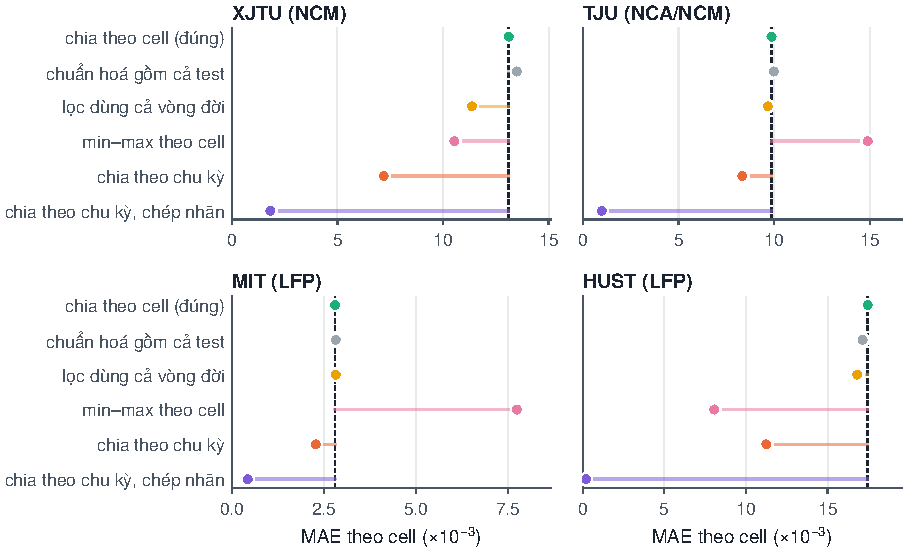
\includegraphics[width=\textwidth]{hinh/fig_leakage.pdf}
\caption[MAE theo cell của cùng một mô hình dưới các cách chia và chuẩn hoá khác nhau]{MAE theo cell của cùng một mô hình
(MLP, 70\,\% nhãn) dưới các cách chia và chuẩn hoá khác nhau; vạch đứt là cách chia đúng (theo cell). Điểm càng lệch trái
so với vạch, sai số càng bị đánh giá thấp giả tạo.}\label{fig:leak}
\end{figure}

\section{PINN bán giám sát và học có nhãn theo lượng nhãn}\label{sec:labels}

Bảng~\ref{tab:big} và Hình~\ref{fig:curvephys} cho sai số của mọi mô hình ở bốn mức nhãn, 5 lần lặp $\times$ 5 fold.

\begin{table}[!htbp]\centering\small
\caption[MAE theo cell của mọi mô hình theo lượng nhãn]{MAE theo cell (×$10^{-3}$) của mọi mô hình theo lượng nhãn (phần trăm số cell có nhãn); in đậm là thấp nhất trong cột của mỗi bộ. Trung bình 5 lần lặp × 5 fold; mỗi cell được kiểm tra 5 lần.}\label{tab:big}
\begin{adjustbox}{max width=\textwidth}\begin{tabular}{llrrrr}\toprule
 & & \multicolumn{4}{c}{MAE theo cell ($\times10^{-3}$) $\downarrow$} \\\cmidrule(lr){3-6}
Bộ & Mô hình & 10\,\% & 30\,\% & 50\,\% & 70\,\% \\\midrule
XJTU & Ridge & 18{,}22 & 15{,}54 & 14{,}81 & 14{,}09 \\
 & GPR & 14{,}85 & 12{,}11 & 14{,}86 & 19{,}18 \\
 & GBDT & \textbf{14{,}49} & \textbf{10{,}85} & \textbf{10{,}19} & \textbf{9{,}51} \\
 & MLP & 24{,}72 & 15{,}95 & 14{,}58 & 12{,}74 \\
 & PINN-sup & 20{,}25 & 14{,}54 & 13{,}21 & 12{,}19 \\
 & PINN hộp đen & 15{,}68 & 14{,}15 & 12{,}82 & 12{,}34 \\
 & PINN-semi & 14{,}93 & 13{,}44 & 13{,}52 & 12{,}19 \\
\addlinespace[3pt]
TJU & Ridge & 23{,}01 & 21{,}60 & 20{,}50 & 20{,}74 \\
 & GPR & 13{,}50 & 9{,}22 & 8{,}01 & 8{,}17 \\
 & GBDT & \textbf{12{,}68} & \textbf{8{,}14} & \textbf{7{,}21} & \textbf{6{,}77} \\
 & MLP & 15{,}50 & 11{,}33 & 9{,}99 & 9{,}64 \\
 & PINN-sup & 14{,}73 & 10{,}67 & 10{,}20 & 10{,}52 \\
 & PINN hộp đen & 13{,}90 & 10{,}91 & 10{,}36 & 10{,}16 \\
 & PINN-semi & 13{,}91 & 10{,}85 & 10{,}46 & 10{,}52 \\
\addlinespace[3pt]
MIT & Ridge & 3{,}53 & 3{,}24 & 3{,}17 & 3{,}13 \\
 & GPR & 3{,}21 & 2{,}14 & 1{,}84 & 1{,}79 \\
 & GBDT & \textbf{3{,}09} & \textbf{1{,}99} & \textbf{1{,}73} & \textbf{1{,}58} \\
 & MLP & 8{,}54 & 3{,}40 & 3{,}04 & 2{,}86 \\
 & PINN-sup & 5{,}34 & 2{,}69 & 2{,}54 & 2{,}44 \\
 & PINN hộp đen & 4{,}19 & 2{,}80 & 2{,}61 & 2{,}54 \\
 & PINN-semi & 3{,}34 & 2{,}58 & 2{,}48 & 2{,}44 \\
\addlinespace[3pt]
HUST & Ridge & \textbf{22{,}88} & 18{,}85 & 18{,}32 & 18{,}10 \\
 & GPR & 28{,}82 & 21{,}24 & 18{,}50 & 17{,}22 \\
 & GBDT & 24{,}13 & 18{,}63 & \textbf{15{,}65} & \textbf{14{,}45} \\
 & MLP & 37{,}95 & 19{,}80 & 17{,}73 & 16{,}94 \\
 & PINN-sup & 31{,}67 & 17{,}82 & 16{,}11 & 15{,}99 \\
 & PINN hộp đen & 24{,}04 & 17{,}49 & 16{,}47 & 15{,}99 \\
 & PINN-semi & 22{,}98 & \textbf{17{,}30} & 16{,}11 & 15{,}99 \\
\bottomrule\end{tabular}\end{adjustbox}\end{table}


\begin{figure}[!htbp]\centering
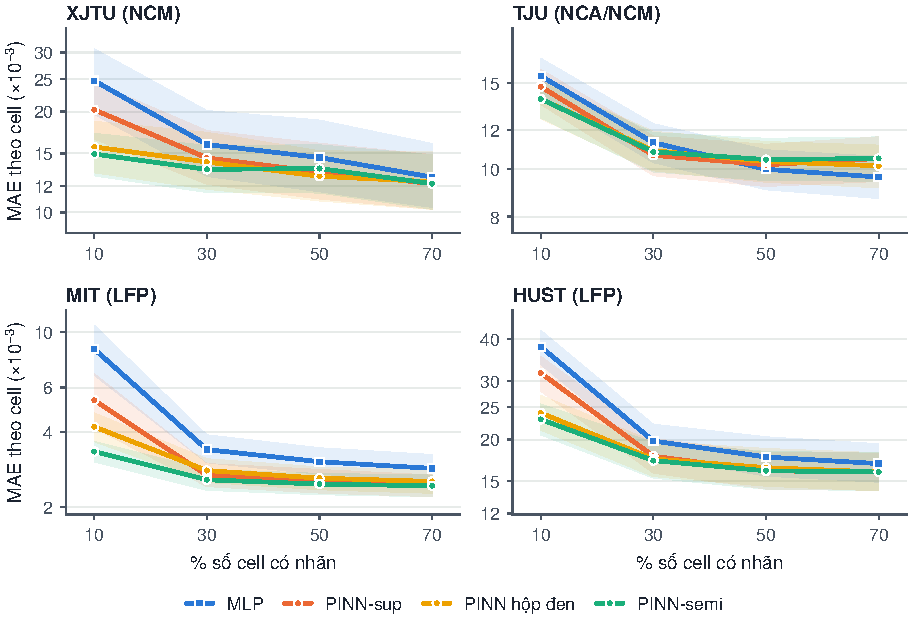
\includegraphics[width=\textwidth]{hinh/fig_curve_physics.pdf}
\caption[MAE theo cell theo lượng nhãn: MLP và các biến thể có vật lý]{MAE theo cell theo lượng nhãn: MLP và các biến thể
có vật lý. Dải là khoảng tin cậy 95\,\% bootstrap theo cell; trục dọc thang log.}\label{fig:curvephys}
\end{figure}

\paragraph{Khi có ít nhãn.} Ở 10\,\% nhãn, PINN-semi có tỉ số MAE so với MLP là XJTU 0{,}60, TJU 0{,}90, MIT 0{,}39,
HUST 0{,}61, thấp hơn có ý nghĩa trên cả bốn bộ (Bảng~\ref{tab:cmp}). Ở mức này mỗi fold chỉ có 6--13 cell có nhãn và
MLP dễ quá khớp; loss vật lý trên các cell không nhãn buộc mạng cho quỹ đạo hợp lý trên chính những cell nó chưa có nhãn.
Quy đổi theo lượng nhãn (nội suy log-tuyến tính giữa các mức), PINN-semi dùng 10\,\% nhãn đạt sai số mà MLP cần XJTU
45\,\%, TJU 17\,\%, MIT 33\,\%, HUST 25\,\% nhãn mới đạt, tức tiết kiệm 1{,}7--4{,}5 lần số nhãn.

\paragraph{Ở 30\,\% nhãn.} PINN-semi thấp hơn MLP có ý nghĩa trên cả bốn bộ, tỉ số 0{,}76 (MIT) tới 0{,}96 (TJU). Với
kiểm định bảo thủ ở mức fold, kết luận chỉ còn đứng vững trên MIT.

\paragraph{Khi có nhiều nhãn.} Ở 70\,\% nhãn mọi cell train đều có nhãn, PINN-semi trùng PINN-sup và vật lý chỉ còn vai
trò chuẩn hoá. Tỉ số so với MLP là XJTU 0{,}96, TJU 1{,}09, MIT 0{,}85, HUST 0{,}94; cải thiện có ý nghĩa trên MIT, còn
trên TJU MLP tốt hơn có ý nghĩa. Trung bình nhân của tỉ số qua bốn bộ đi từ 0{,}60 (10\,\%) qua 0{,}86 (30\,\%), 0{,}92
(50\,\%) tới 0{,}96 (70\,\%): nhãn càng đủ, ràng buộc vật lý càng ít thông tin mới.

\paragraph{So với các mô hình học có nhãn khác.} GBDT là đối thủ mạnh nhất: nó thấp hơn PINN-semi có ý nghĩa ở 10\,\%
(TJU) và ở 30, 50, 70\,\% (XJTU, TJU, MIT); PINN-semi chỉ thấp hơn GBDT có ý nghĩa ở HUST 30\,\%. GPR kém GBDT ở 16/16
trường hợp bộ $\times$ mức nhãn nhưng vẫn thấp hơn PINN-semi ở 10/16. Ridge tốt hơn MLP ở 10\,\% nhãn trên XJTU, MIT và
HUST nhưng cải thiện chậm khi thêm nhãn. Như vậy vật lý cải thiện rõ mạng nơ-ron khi ít nhãn và đưa nó tới gần mô hình
cây ở 10\,\% nhãn (tỉ số so với GBDT 0{,}95--1{,}10), nhưng PINN-semi đơn lẻ chưa vượt được GBDT.

\begin{table}[!htbp]\centering\scriptsize
\caption[Tỉ số MAE của PINN-semi so với MLP và GBDT]{Tỉ số MAE theo cell của PINN-semi so với MLP và GBDT ở từng mức nhãn (nhỏ hơn 1: PINN-semi tốt hơn). $^{*}$: $p_\text{Holm} < 0{,}05$ theo cell; $^{\dagger}$: còn có ý nghĩa với kiểm định bảo thủ mức fold.}\label{tab:cmp}
\begin{adjustbox}{max width=\textwidth}\begin{tabular}{llrrrrrr}\toprule
Bộ & Nhãn & so với MLP: tỉ số [KTC] & cell tốt hơn & $p_\text{Holm}$ & so với GBDT: tỉ số [KTC] & cell tốt hơn & $p_\text{Holm}$ \\\midrule
XJTU & 10\,\% & 0{,}60 [0{,}54; 0{,}68]$^{*}$ & 91\,\% & $<10^{-4}$ & 1{,}03 [0{,}93; 1{,}15] & 47\,\% & 0{,}8210 \\
 & 30\,\% & 0{,}84 [0{,}76; 0{,}93]$^{*}$ & 65\,\% & 0{,}0047 & 1{,}24 [1{,}11; 1{,}42]$^{*}$ & 31\,\% & 0{,}0004 \\
 & 50\,\% & 0{,}93 [0{,}81; 1{,}06] & 45\,\% & 0{,}7502 & 1{,}33 [1{,}17; 1{,}53]$^{*}$ & 20\,\% & $<10^{-4}$ \\
 & 70\,\% & 0{,}96 [0{,}90; 1{,}02] & 53\,\% & 0{,}4712 & 1{,}28 [1{,}11; 1{,}54]$^{*}$ & 33\,\% & 0{,}0010 \\
TJU & 10\,\% & 0{,}90 [0{,}87; 0{,}93]$^{*}$ & 75\,\% & $<10^{-4}$ & 1{,}10 [1{,}02; 1{,}18]$^{*}$ & 38\,\% & 0{,}0340 \\
 & 30\,\% & 0{,}96 [0{,}93; 0{,}99]$^{*}$ & 68\,\% & 0{,}0041 & 1{,}33 [1{,}24; 1{,}44]$^{*}$ & 28\,\% & $<10^{-4}$ \\
 & 50\,\% & 1{,}05 [1{,}01; 1{,}09] & 43\,\% & 0{,}2363 & 1{,}45 [1{,}33; 1{,}58]$^{*}$$^{\dagger}$ & 22\,\% & $<10^{-4}$ \\
 & 70\,\% & 1{,}09 [1{,}04; 1{,}14]$^{*}$ & 41\,\% & 0{,}0086 & 1{,}55 [1{,}40; 1{,}72]$^{*}$$^{\dagger}$ & 20\,\% & $<10^{-4}$ \\
MIT & 10\,\% & 0{,}39 [0{,}32; 0{,}48]$^{*}$ & 90\,\% & $<10^{-4}$ & 1{,}08 [1{,}00; 1{,}16] & 45\,\% & 0{,}1991 \\
 & 30\,\% & 0{,}76 [0{,}69; 0{,}83]$^{*}$$^{\dagger}$ & 82\,\% & $<10^{-4}$ & 1{,}30 [1{,}21; 1{,}40]$^{*}$$^{\dagger}$ & 18\,\% & $<10^{-4}$ \\
 & 50\,\% & 0{,}81 [0{,}75; 0{,}88]$^{*}$ & 79\,\% & $<10^{-4}$ & 1{,}43 [1{,}34; 1{,}54]$^{*}$$^{\dagger}$ & 9\,\% & $<10^{-4}$ \\
 & 70\,\% & 0{,}85 [0{,}79; 0{,}92]$^{*}$ & 74\,\% & $<10^{-4}$ & 1{,}54 [1{,}44; 1{,}67]$^{*}$$^{\dagger}$ & 6\,\% & $<10^{-4}$ \\
HUST & 10\,\% & 0{,}61 [0{,}55; 0{,}67]$^{*}$ & 92\,\% & $<10^{-4}$ & 0{,}95 [0{,}89; 1{,}02] & 61\,\% & 0{,}0720 \\
 & 30\,\% & 0{,}87 [0{,}82; 0{,}92]$^{*}$ & 71\,\% & $<10^{-4}$ & 0{,}93 [0{,}86; 1{,}00]$^{*}$ & 69\,\% & 0{,}0042 \\
 & 50\,\% & 0{,}91 [0{,}87; 0{,}95]$^{*}$ & 68\,\% & 0{,}0008 & 1{,}03 [0{,}95; 1{,}12] & 56\,\% & 0{,}9939 \\
 & 70\,\% & 0{,}94 [0{,}90; 0{,}99] & 65\,\% & 0{,}0526 & 1{,}11 [1{,}01; 1{,}22] & 43\,\% & 0{,}0923 \\
\bottomrule\end{tabular}\end{adjustbox}\end{table}


\section{Lợi ích của PINN-semi đến từ đâu}\label{sec:source}

\begin{table}[!htbp]\centering\small
\caption[Tách nguồn gốc lợi ích ở 30\,\% nhãn]{Tách nguồn gốc lợi ích ở 30\,\% nhãn: MAE theo cell (×$10^{-3}$), trong ngoặc là tỉ số so với MLP.}\label{tab:source}
\begin{adjustbox}{max width=\textwidth}\begin{tabular}{lrrrr}\toprule
Mô hình (30\,\% nhãn) & XJTU & TJU & MIT & HUST \\\midrule
MLP & 15{,}95 & 11{,}33 & 3{,}40 & 19{,}80 \\
PINN-sup & 14{,}54 (0{,}91) & 10{,}67 (0{,}94) & 2{,}69 (0{,}79) & 17{,}82 (0{,}90) \\
chỉ đơn điệu & 14{,}13 (0{,}89) & 11{,}00 (0{,}97) & 2{,}86 (0{,}84) & 17{,}41 (0{,}88) \\
PINN-semi (Euler) & 13{,}37 (0{,}84) & 11{,}31 (1{,}00) & 3{,}01 (0{,}89) & 17{,}49 (0{,}88) \\
PINN hộp đen & 14{,}15 (0{,}89) & 10{,}91 (0{,}96) & 2{,}80 (0{,}83) & 17{,}49 (0{,}88) \\
PINN-semi & 13{,}44 (0{,}84) & 10{,}85 (0{,}96) & 2{,}58 (0{,}76) & 17{,}30 (0{,}87) \\
\bottomrule\end{tabular}\end{adjustbox}\end{table}


Bảng~\ref{tab:source} tách lợi ích ở 30\,\% nhãn. Chỉ riêng ràng buộc đơn điệu đã mang lại 62--95\,\% mức giảm sai số
(thang log) của PINN-semi so với MLP; bỏ $\mathcal{L}_\text{ode}$ và $\mathcal{L}_\text{range}$ làm MAE bằng 1{,}01--1{,}11
lần PINN-semi đầy đủ, lớn nhất ở MIT. Ở 10\,\% nhãn, phần do áp loss vật lý lên cell không nhãn (PINN-semi so với
PINN-sup, tỉ số XJTU 0{,}74, TJU 0{,}94, MIT 0{,}62, HUST 0{,}73) chiếm 50--64\,\% mức giảm sai số so với MLP. Động học
xám tốt hơn động học hộp đen kiểu PINN4SOH có ý nghĩa ở 4 trong 16 trường hợp, kém hơn có ý nghĩa ở 1; ở 30\,\% nhãn sai
số của PINN hộp đen gần như trùng biến thể chỉ đơn điệu (chênh không quá 2\,\%), phù hợp với giả thuyết rằng khi $G$ nhận
cả $u_t$, mạng học được $G \approx u_t$ và phần dư động học bị thoả mãn tầm thường.

\section{Mô hình chuỗi thời gian, GBDT và PINN-lai}\label{sec:e20res}

Bảng~\ref{tab:allmae} đặt bốn mô hình học sâu của đề cương cạnh GBDT, PINN-semi và PINN-lai, cùng fold, cùng cell có nhãn,
3 lần lặp.

\begin{table}[!htbp]\centering\footnotesize
\caption[MAE theo cell của mọi mô hình chính]{MAE theo cell ($\times10^{-3}$) trên tập kiểm tra của mọi mô hình chính, 3 lần lặp $\times$ 5 fold, cùng fold và cell có nhãn; in đậm là thấp nhất mỗi hàng. PINN-lai là cấu hình cố định ($\omega = \tfrac12$, $w = 10$), chốt trước khi đọc tập kiểm tra. HiPINN-lai là PINN-lai có thêm đặc trưng lịch sử của đặc trưng sạc ở những fold mà tập xác thực chọn; trên bộ không có dạng lịch sử nào được chọn (MIT), hai cột trùng nhau. HiPINN-lai là phân tích hậu kiểm (\Cref{sec:pinnlai}).}\label{tab:allmae}
\begin{adjustbox}{max width=\textwidth}\begin{tabular}{llrrrrrrrr}\toprule
 & & \multicolumn{8}{c}{MAE theo cell ($\times10^{-3}$) $\downarrow$} \\\cmidrule(lr){3-10}
Bộ & Nhãn & MLP & CNN & LSTM & Transformer & GBDT & PINN-semi & PINN-lai & HiPINN-lai \\\midrule
XJTU & 10\,\% & 23{,}27 & 16{,}01 & 16{,}62 & 17{,}63 & 14{,}01 & 14{,}65 & \textbf{12{,}83} & 13{,}34 \\
 & 30\,\% & 15{,}61 & 12{,}68 & 13{,}98 & 13{,}71 & \textbf{10{,}87} & 13{,}35 & 11{,}43 & 11{,}46 \\
 & 50\,\% & 14{,}10 & 11{,}69 & 11{,}98 & 12{,}05 & \textbf{10{,}18} & 13{,}20 & 10{,}65 & 10{,}63 \\
 & 70\,\% & 12{,}48 & 10{,}98 & 10{,}50 & 10{,}99 & \textbf{9{,}64} & 12{,}53 & 10{,}00 & 10{,}00 \\
TJU & 10\,\% & 15{,}81 & 14{,}22 & 13{,}08 & 14{,}14 & 12{,}60 & 14{,}01 & 11{,}79 & \textbf{11{,}73} \\
 & 30\,\% & 11{,}71 & 8{,}89 & 8{,}69 & 9{,}89 & \textbf{8{,}06} & 11{,}39 & 8{,}52 & 8{,}19 \\
 & 50\,\% & 9{,}96 & 7{,}31 & 7{,}24 & 9{,}31 & \textbf{7{,}17} & 10{,}74 & 7{,}77 & 7{,}36 \\
 & 70\,\% & 9{,}71 & 7{,}36 & 7{,}09 & 8{,}96 & \textbf{6{,}96} & 10{,}80 & 7{,}76 & 7{,}25 \\
MIT & 10\,\% & 9{,}02 & 3{,}30 & 3{,}26 & 3{,}87 & 3{,}15 & 3{,}29 & \textbf{2{,}52} & \textbf{2{,}52} \\
 & 30\,\% & 3{,}39 & 2{,}18 & 2{,}18 & 2{,}77 & 1{,}97 & 2{,}50 & \textbf{1{,}79} & \textbf{1{,}79} \\
 & 50\,\% & 3{,}06 & 1{,}99 & 2{,}04 & 2{,}71 & 1{,}74 & 2{,}45 & \textbf{1{,}67} & \textbf{1{,}67} \\
 & 70\,\% & 2{,}85 & 1{,}93 & 1{,}99 & 2{,}59 & \textbf{1{,}59} & 2{,}38 & \textbf{1{,}59} & \textbf{1{,}59} \\
HUST & 10\,\% & 41{,}62 & 22{,}77 & 24{,}51 & 21{,}95 & 23{,}84 & 22{,}76 & 20{,}52 & \textbf{20{,}08} \\
 & 30\,\% & 20{,}00 & 17{,}42 & 17{,}14 & 17{,}45 & 18{,}73 & 17{,}10 & 16{,}19 & \textbf{15{,}43} \\
 & 50\,\% & 18{,}13 & 15{,}04 & 15{,}52 & 16{,}00 & 15{,}82 & 16{,}42 & 14{,}29 & \textbf{13{,}24} \\
 & 70\,\% & 17{,}19 & 14{,}19 & 14{,}76 & 14{,}93 & 14{,}60 & 16{,}38 & 13{,}78 & \textbf{12{,}33} \\
\bottomrule\end{tabular}\end{adjustbox}\end{table}


\paragraph{Bốn mô hình học sâu.} So với MLP, tỉ số MAE của CNN là 0{,}37--0{,}90, của LSTM 0{,}36--0{,}90, của Transformer
0{,}43--0{,}93; mô hình chuỗi thấp hơn MLP có ý nghĩa ở 42/48 phép so. Nhìn nhiều chu kỳ cho mô hình thấy xu thế của đặc
trưng sạc và làm trung bình nhiễu đo của từng chu kỳ. Trong ba mô hình chuỗi, LSTM thấp nhất ở 8/16 trường hợp. Mô hình
chuỗi tốt nhất thấp hơn GBDT ở 4/16 trường hợp (mọi mức nhãn trên HUST) và thấp hơn PINN-semi ở 14/16.

\paragraph{PINN-lai.} Cấu hình chọn trên validation của lần lặp 0: kết hợp với GBDT cho mức giảm lớn nhất (tỉ số
validation so với PINN-semi 0{,}843 ở 10\,\% và 0{,}804 ở 50\,\% nhãn), nhóm ba mạng giảm vừa phải (0{,}963), còn ba hướng
làm sai số tăng: ràng buộc đơn điệu mạnh hơn (1{,}065), thêm phần dư Euler (1{,}289) và đặc trưng tương đối (1{,}692).
Các tỉ số sau là của cấu hình cố định ($\omega = \tfrac12$, $w = 10$); cột PINN-lai của Bảng~\ref{tab:allmae} là bản có
trọng số ghép và cửa sổ lọc chọn lại trên validation của đủ 3 lần lặp, đặt ra sau khi đã xem test (hậu kiểm), có sai số
bằng 0{,}92--1{,}00 lần bản cố định. Trên test, PINN-lai thấp hơn PINN-semi ở 16/16 trường hợp, cả 16 có ý nghĩa, tỉ số
0{,}67--0{,}95; thấp hơn GBDT ở 10/16
(8 có ý nghĩa), và ở 10\,\% nhãn thấp hơn GBDT có ý nghĩa trên cả bốn bộ; GBDT chỉ còn tốt hơn có ý nghĩa ở TJU 70\,\%.
PINN-lai thấp hơn cả ba mô hình chuỗi ở 47/48 phép so (40 có ý nghĩa). Trên hai mức nhãn dùng khi phát triển, tỉ số so với
PINN-semi trên test là 0{,}805, gần 0{,}823 trên validation, nên việc chọn trên validation không làm kết quả test lạc quan
đáng kể. Tính trung bình nhân trên 16 trường hợp, nhóm ba mạng đưa tỉ số so với PINN-semi xuống 0{,}961, kết hợp với GBDT
xuống 0{,}798, bộ lọc xuống 0{,}793: bước kết hợp mang phần lớn lợi ích, vì lệch mức theo cell của nhóm PINN và của GBDT
chỉ tương quan vừa (Pearson 0{,}50--0{,}80) và ngược dấu nhau ở 16--31\,\% số cell. Áp cùng công thức với ba MLP thay cho
ba PINN-semi, PINN-lai tốt hơn có ý nghĩa ở 7/16 trường hợp và kém hơn ở 1; tỉ số trung bình nhân 0{,}716 ở 10\,\% và
1{,}002 ở 70\,\% nhãn: phần vật lý vẫn đóng góp khi ít nhãn.

\paragraph{RMSE, MAPE và $R^2$.} Ở 30\,\% nhãn (Bảng~\ref{tab:allrm}), RMSE và MAPE cũng thấp nhất ở PINN-lai hoặc mô hình
cuối và cao nhất ở MLP trên cả bốn bộ. Mô hình có MAE thấp nhất cũng có $R^2$ cao nhất ở 14/16 trường hợp; $R^2$ tính từ chu
kỳ 10 của PINN-lai ở 30\,\% nhãn là 0{,}867--0{,}992.

\begin{table}[!htbp]\centering\footnotesize
\caption[RMSE và MAPE của mọi mô hình chính ở 30\,\% nhãn]{Ở 30\,\% nhãn: RMSE theo cell ($\times10^{-3}$) và MAPE (\%, tính chung mọi chu kỳ) trên tập kiểm tra; in đậm là thấp nhất mỗi cột. PINN-lai và HiPINN-lai như ở Bảng~\ref{tab:allmae}.}\label{tab:allrm}
\begin{adjustbox}{max width=\textwidth}\begin{tabular}{lrrrrrrrr}\toprule
 & \multicolumn{2}{c}{XJTU} & \multicolumn{2}{c}{TJU} & \multicolumn{2}{c}{MIT} & \multicolumn{2}{c}{HUST} \\\cmidrule(lr){2-3}\cmidrule(lr){4-5}\cmidrule(lr){6-7}\cmidrule(lr){8-9}
Mô hình & RMSE $\downarrow$ & MAPE $\downarrow$ & RMSE $\downarrow$ & MAPE $\downarrow$ & RMSE $\downarrow$ & MAPE $\downarrow$ & RMSE $\downarrow$ & MAPE $\downarrow$ \\\midrule
MLP & 23{,}10 & 1{,}47 & 13{,}94 & 1{,}20 & 4{,}65 & 0{,}41 & 26{,}07 & 2{,}12 \\
CNN & 16{,}11 & 1{,}27 & 10{,}60 & 0{,}94 & 3{,}04 & 0{,}23 & 24{,}04 & 1{,}89 \\
LSTM & 17{,}91 & 1{,}32 & 10{,}27 & 0{,}94 & 3{,}05 & 0{,}23 & 23{,}45 & 1{,}85 \\
Transformer & 17{,}39 & 1{,}37 & 11{,}72 & 1{,}04 & 3{,}72 & 0{,}29 & 23{,}17 & 1{,}87 \\
GBDT & \textbf{14{,}37} & 1{,}19 & 9{,}74 & 0{,}90 & 2{,}93 & 0{,}21 & 25{,}98 & 2{,}04 \\
PINN-semi & 19{,}42 & 1{,}32 & 13{,}54 & 1{,}16 & 3{,}34 & 0{,}28 & 22{,}84 & 1{,}83 \\
PINN-lai & 15{,}80 & 1{,}18 & 10{,}14 & 0{,}91 & \textbf{2{,}46} & \textbf{0{,}19} & 22{,}29 & 1{,}75 \\
HiPINN-lai & 15{,}56 & \textbf{1{,}17} & \textbf{9{,}70} & \textbf{0{,}88} & \textbf{2{,}46} & \textbf{0{,}19} & \textbf{21{,}74} & \textbf{1{,}67} \\
\bottomrule\end{tabular}\end{adjustbox}\end{table}


\section{Khoảng dự đoán}\label{sec:conformal}

PINN-lai được gắn khoảng dự đoán 90\,\% bằng dự đoán phù hợp tách tập, hiệu chỉnh trên validation của từng fold; dạng thích
nghi chia phần dư cho độ vênh giữa nhóm PINN và GBDT. Độ phủ thực tế trên test là 84{,}9--92{,}6\,\% với độ rộng cố định và
86{,}3--92{,}9\,\% với độ rộng thích nghi, trung bình 88{,}8\,\%. Độ rộng trung bình của dạng thích nghi là 0{,}65--10{,}19\,\%
SOH. Với độ rộng thích nghi, 14--25\,\% số cell có độ phủ dưới 80\,\%: đó là các cell bị lệch mức cả đời.

\section{Ngân sách đo và cập nhật khi dùng}\label{sec:budgetres}

\begin{table}[!htbp]\centering\small
\caption[MAE theo cell theo ngân sách đo dung lượng]{MAE theo cell ($\times10^{-3}$) trên test, trung bình 3 lần lặp; trong ngoặc là phần trăm số chu kỳ của cell train có đo dung lượng (70\,\% số cell là toàn bộ). Hai cột đo thưa: mọi cell train được đo ở chu kỳ đầu, sau mỗi $qL$ chu kỳ và ở chu kỳ cuối. Cột cuối: đo thêm cell test theo cùng lịch, cập nhật bằng bộ lọc Kalman, sai số trên các chu kỳ không được đo. In đậm là thấp nhất trong năm cột đầu của mỗi hàng; cột cuối có đo thêm cell test nên không so cùng.}\label{tab:e28}
\begin{adjustbox}{max width=\textwidth}\begin{tabular}{lrrrrrr}\toprule
 & \multicolumn{6}{c}{MAE theo cell ($\times10^{-3}$) $\downarrow$} \\\cmidrule(lr){2-7}
Bộ & \begin{tabular}[b]{@{}r@{}}PINN-lai,\\30\,\% cell\end{tabular} & \begin{tabular}[b]{@{}r@{}}PINN-lai,\\70\,\% cell\end{tabular} & \begin{tabular}[b]{@{}r@{}}GBDT,\\70\,\% cell\end{tabular} & \begin{tabular}[b]{@{}r@{}}PINN-lai, đo\\mỗi $0{,}1L$\end{tabular} & \begin{tabular}[b]{@{}r@{}}PINN-lai, đo\\mỗi $0{,}05L$\end{tabular} & \begin{tabular}[b]{@{}r@{}}đo cả cell mới\\mỗi $0{,}1L$\end{tabular} \\\midrule
XJTU & 11{,}43 (44{,}1) & 10{,}00 & \textbf{9{,}64} & 10{,}51 (3{,}2) & 10{,}28 (6{,}0) & 7{,}46 \\
TJU & 8{,}52 (42{,}6) & 7{,}76 & \textbf{6{,}96} & 8{,}28 (3{,}1) & 7{,}54 (5{,}9) & 4{,}13 \\
MIT & 1{,}79 (42{,}7) & \textbf{1{,}59} & \textbf{1{,}59} & 1{,}91 (1{,}9) & 1{,}67 (3{,}6) & 1{,}18 \\
HUST & 16{,}19 (43{,}1) & \textbf{13{,}78} & 14{,}60 & 13{,}87 (0{,}6) & \textbf{13{,}78} (1{,}2) & 5{,}00 \\
\bottomrule\end{tabular}\end{adjustbox}\end{table}


\begin{figure}[!htbp]\centering
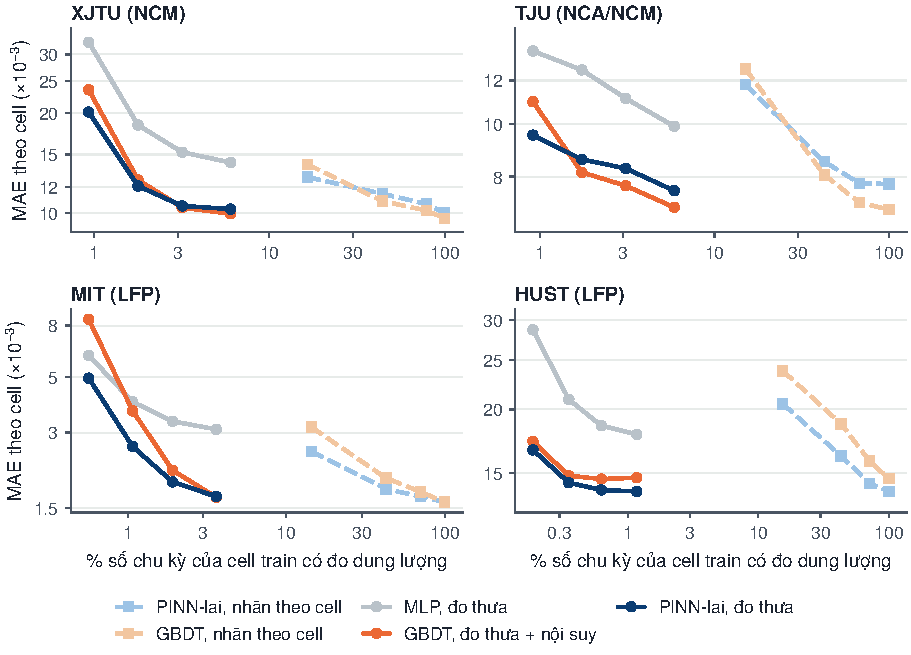
\includegraphics[width=\textwidth]{hinh/fig_e28_budget.pdf}
\caption[MAE theo phần trăm số chu kỳ của cell train có đo dung lượng]{MAE theo cell trên test theo phần trăm số chu kỳ
của cell train có đo dung lượng (hai trục thang log). Nét đứt: nhãn theo cell (10, 30, 50, 70\,\% số cell có nhãn đầy
đủ); nét liền: đo thưa mọi cell train theo lịch $qL$, $q$ = 0{,}5; 0{,}2; 0{,}1; 0{,}05.}\label{fig:e28}
\end{figure}

Gắn nhãn đầy đủ cho 30\,\% số cell tương ứng 43--44\,\% số chu kỳ train. Đo mỗi $0{,}05L$ chu kỳ trên mọi cell chỉ dùng
1{,}2--6{,}0\,\% số chu kỳ, ít hơn 7--37 lần, nhưng PINN-lai học theo cách này có MAE bằng 0{,}85--0{,}93 lần PINN-lai học
với 30\,\% số cell, thấp hơn có ý nghĩa trên cả bốn bộ (Bảng~\ref{tab:e28}, Hình~\ref{fig:e28}). So với 70\,\% số cell, tỉ
số là 0{,}97--1{,}05: tốt hơn có ý nghĩa ở TJU, kém hơn có ý nghĩa ở MIT. Lý do là phần lớn sai số là lệch mức riêng của
từng cell, mô hình chỉ học được khi thấy nhãn của chính cell đó, còn các chu kỳ liền nhau của một cell gần như lặp lại
thông tin của nhau. Khi cell mới cũng được đo theo lịch $0{,}1L$ (1--3\,\% số chu kỳ của nó) và ước lượng được cập nhật
bằng bộ lọc Kalman, MAE trên các chu kỳ không được đo còn 1{,}2--7{,}5 ($\times10^{-3}$), bằng 0{,}34--0{,}77 lần GBDT học
với 70\,\% số cell có nhãn đầy đủ nhưng không đo cell mới. Mô hình cập nhật học thẳng thay đổi SOH kể từ lần đo gần nhất
thấp hơn bộ lọc Kalman ở 47/48 trường hợp bộ $\times$ mức nhãn $\times$ lịch đo (tỉ số 0{,}15--1{,}06) và thấp hơn việc giữ
nguyên giá trị đo gần nhất ở 48/48 (tỉ số 0{,}07--0{,}53).

\section{Dự báo SOH tương lai và RUL}\label{sec:forecastres}

\begin{table}[!htbp]\centering\small
\caption[MAE của SOH dự báo ở ba tầm]{MAE theo cell ($\times10^{-3}$) của SOH dự báo ở ba tầm, kịch bản lịch sử ước lượng (không đo dung lượng cell test); in đậm là thấp nhất. Hai cột cuối: mô hình kết hợp khi lịch sử là dung lượng đo, và sai số của mô hình kết hợp quy ra dung lượng (mAh) ở kịch bản ước lượng.}\label{tab:e22soh}
\begin{adjustbox}{max width=\textwidth}\begin{tabular}{llrrrrrrrr}\toprule
Bộ & Tầm & Giữ nguyên & Tuyến tính & Vật lý theo cell & GBDT & PINN-dự báo & Kết hợp & Kết hợp, đo & Kết hợp (mAh) \\\midrule
XJTU & 0{,}1$L$ & 14{,}2 & 12{,}2 & 23{,}4 & \textbf{10{,}8} & 12{,}4 & 10{,}8 & 5{,}4 & 22 \\
 & 0{,}25$L$ & 36{,}2 & 28{,}8 & 39{,}6 & \textbf{16{,}2} & 23{,}5 & 18{,}8 & 13{,}8 & 38 \\
 & 0{,}5$L$ & 70{,}2 & 58{,}8 & 62{,}3 & \textbf{26{,}5} & 32{,}3 & 28{,}4 & 22{,}5 & 57 \\
TJU & 0{,}1$L$ & 15{,}0 & 11{,}0 & 9{,}9 & 9{,}0 & \textbf{8{,}1} & 8{,}4 & 3{,}0 & 29 \\
 & 0{,}25$L$ & 38{,}3 & 23{,}5 & 18{,}5 & 12{,}9 & 13{,}1 & \textbf{12{,}0} & 7{,}2 & 42 \\
 & 0{,}5$L$ & 56{,}5 & 18{,}9 & 17{,}7 & \textbf{10{,}7} & 13{,}0 & 12{,}1 & 11{,}5 & 42 \\
MIT & 0{,}1$L$ & 8{,}9 & 4{,}3 & \textbf{3{,}9} & 5{,}7 & 7{,}2 & 5{,}5 & 4{,}9 & 6 \\
 & 0{,}25$L$ & 26{,}2 & 15{,}3 & 14{,}7 & \textbf{7{,}9} & 10{,}7 & 8{,}8 & 8{,}0 & 10 \\
 & 0{,}5$L$ & 53{,}0 & 39{,}7 & 37{,}6 & \textbf{17{,}0} & 19{,}6 & 17{,}8 & 16{,}8 & 20 \\
HUST & 0{,}1$L$ & 22{,}2 & \textbf{13{,}0} & 35{,}9 & 14{,}3 & 14{,}2 & 13{,}7 & 2{,}8 & 15 \\
 & 0{,}25$L$ & 66{,}3 & 30{,}0 & 103{,}0 & 25{,}4 & 25{,}6 & \textbf{24{,}9} & 8{,}3 & 27 \\
 & 0{,}5$L$ & 136{,}6 & 69{,}1 & 111{,}1 & \textbf{32{,}0} & 37{,}1 & 33{,}1 & 20{,}5 & 36 \\
\bottomrule\end{tabular}\end{adjustbox}\end{table}

\begin{table}[!htbp]\centering\small
\caption[MAE của RUL dự báo]{MAE của RUL (chu kỳ), kịch bản lịch sử ước lượng, trung bình qua gốc ở 25, 50, 75\,\% đời; cột RUL thực là trung bình RUL thật tại các gốc. Ba cột cuối của mô hình kết hợp: MAE khi lịch sử là dung lượng đo, tỉ lệ dự báo nằm trong $\pm20\,\%$ RUL thật và độ phủ thực tế của khoảng RUL 90\,\%.}\label{tab:e22rul}
\begin{adjustbox}{max width=\textwidth}\begin{tabular}{lrrrrrrrrr}\toprule
Bộ & RUL thực & Tuyến tính & Vật lý theo cell & GBDT & PINN-dự báo & Kết hợp & Kết hợp, đo & Trong $\pm20\,\%$ & Độ phủ khoảng \\\midrule
XJTU & 231 & 529 & 499 & 145 & 99 & \textbf{96} & 85 & 38\,\% & 70\,\% \\
TJU & 131 & 50 & 45 & 23 & 23 & \textbf{20} & 14 & 65\,\% & 84\,\% \\
MIT & 344 & 836 & 877 & 131 & 118 & \textbf{113} & 112 & 48\,\% & 67\,\% \\
HUST & 923 & 1354 & 1360 & 312 & \textbf{216} & 218 & 104 & 52\,\% & 65\,\% \\
\bottomrule\end{tabular}\end{adjustbox}\end{table}


Khi cell test không được đo dung lượng lần nào và lịch sử SOH là ước lượng PINN-lai, mô hình kết hợp dự báo SOH trên toàn
bộ phần đời còn lại với sai số chỉ bằng 0{,}21--0{,}46 lần dự báo giữ nguyên, 0{,}39--0{,}60 lần ngoại suy tuyến tính và
0{,}27--0{,}58 lần khớp vật lý theo cell, khác biệt có ý nghĩa trên cả bốn bộ (Bảng~\ref{tab:e22soh}). Giữa các mô hình học
từ nhiều cell khác biệt nhỏ hơn: so với GBDT tỉ số là 0{,}91--1{,}06. Quy ra dung lượng, sai số của mô hình kết hợp ở tầm
$0{,}5L$ là 20--57\,mAh. Về RUL (Bảng~\ref{tab:e22rul}), GBDT không ngoại suy được ra ngoài miền tầm dự báo đã học nên cắt
ngưỡng quá muộn; sai số RUL của nó gấp 1{,}1--1{,}5 lần mô hình kết hợp, và mô hình kết hợp tốt hơn GBDT có ý nghĩa trên cả
bốn bộ. Dấu của $\lambda$ học được khớp hình dạng quỹ đạo: dương ở 83--100\,\% số gốc của XJTU, MIT, HUST (có đầu gối),
còn ở TJU trung vị $\lambda$ âm (suy giảm chậm dần).

\begin{figure}[!htbp]\centering
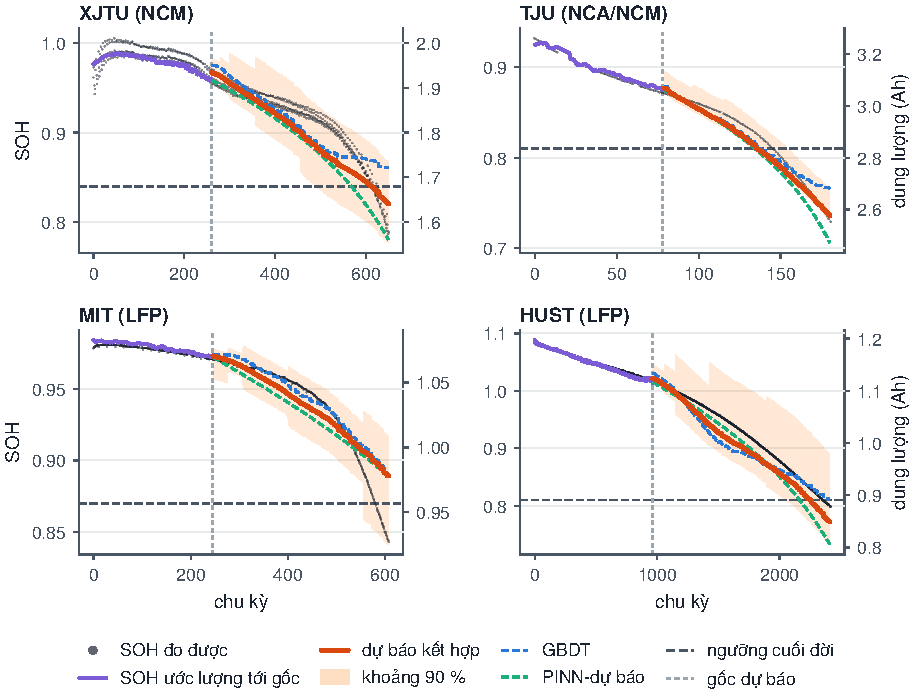
\includegraphics[width=\textwidth]{hinh/fig_e22_traj.pdf}
\caption[Dự báo cho một cell test mỗi bộ]{Dự báo cho một cell test mỗi bộ (lần lặp 0, gốc ở 40\,\% đời, cell có sai số ở
trung vị): lịch sử SOH ước lượng tới gốc, dự báo của GBDT, PINN-dự báo và mô hình kết hợp kèm khoảng 90\,\%; trục phải là
dung lượng (Ah).}\label{fig:e22traj}
\end{figure}

%% ============================================================================ CHƯƠNG 6
\chapter{Đối chiếu với các bài báo đã công bố}\label{ch:sosanh}

\subsection{Mốc so sánh}
Trên bốn bộ dữ liệu này, công trình cùng bài toán, cùng đầu vào và có công bố sai số theo từng nhóm cell kiểm tra là PINN4SOH~\cite{wang2024}. Bài đó còn báo cáo hai mô hình đối chứng MLP và CNN trên cùng các nhóm. Các bài công bố bộ dữ liệu gốc giải bài toán khác hoặc dùng đầu vào khác: Severson và cộng sự~\cite{severson2019} dự đoán tuổi thọ của cả cell từ các chu kỳ đầu, Zhu và cộng sự~\cite{zhu2022} dùng điện áp hồi phục sau sạc, Ma và cộng sự~\cite{ma2022} dùng học chuyển giao với cách chia riêng. Vì cách chia và đầu vào khác nhau, sai số của các bài đó không so trực tiếp được với đồ án, và báo cáo không trích chúng. Mọi so sánh dưới đây dùng đúng 39 nhóm đánh giá của bài, dựng lại từ nhật ký huấn luyện công bố kèm mã: mỗi nhóm thí nghiệm (batch) của XJTU và TJU là một nhóm đánh giá ở chế độ đầy đủ, một nhóm cho MIT (23 cell kiểm tra) và cho HUST (20 cell kiểm tra), và các nhóm ít mẫu $K = 1, \dots, 4$ của XJTU và HUST. Sai số tính đúng như bài: MAE từng cell kiểm tra, trung bình qua lần chạy, qua cell, qua nhóm. PINN-lai của đồ án chạy với hai cách tiền xử lý: bản sao tiền xử lý của bài (có rò rỉ, chỉ để so cùng điều kiện) và tiền xử lý không rò rỉ của đồ án. Bảng~\ref{tab:pub} và \Cref{fig:bench} tập hợp các con số.

\begin{table}[!htbp]\centering\small\setlength{\tabcolsep}{5pt}
\caption[So với PINN4SOH trên đúng cách chia của bài]{MAE theo cell ($\times10^{-3}$) trên đúng 39 nhóm đánh giá của bài PINN4SOH, trung bình qua cell kiểm tra, lần chạy và nhóm như bài; $K$ là số cell có nhãn trong thí nghiệm ít mẫu. Ba cột đầu là số công bố của bài cho PINN4SOH và hai mô hình đối chứng MLP, CNN của bài. Cột chạy lại: mã gốc của bài chạy trên đúng các nhóm đó, siêu tham số theo nhật ký của bài, 10 lần mỗi nhóm. Hai cột cuối: PINN-lai của đồ án (3 hạt giống) với tiền xử lý của bài, cùng điều kiện với các cột trước, và với tiền xử lý không rò rỉ. In đậm: thấp nhất trong năm cột cùng điều kiện. $^{*}$/$^{\dagger}$: PINN-lai với tiền xử lý của bài thấp hơn/cao hơn có ý nghĩa thống kê so với mã gốc chạy lại (Wilcoxon ghép cặp theo cell kiểm tra, Holm qua 12 hàng).}\label{tab:pub}
\begin{adjustbox}{max width=\textwidth}\begin{tabular}{llrrrrrr}\toprule
 & & \multicolumn{6}{c}{MAE theo cell ($\times10^{-3}$) $\downarrow$} \\\cmidrule(lr){3-8}
 & & \multicolumn{3}{c}{số công bố của bài} & PINN4SOH & \multicolumn{2}{c}{PINN-lai của đồ án} \\\cmidrule(lr){3-5}\cmidrule(lr){6-6}\cmidrule(lr){7-8}
Bộ & Chế độ & PINN4SOH & MLP & CNN & chạy lại & tiền xử lý của bài & không rò rỉ \\\midrule
XJTU & đầy đủ & 7{,}85 & 21{,}02 & 21{,}19 & 8{,}66 & \textbf{6{,}62} & 7{,}81 \\
TJU & đầy đủ & 9{,}79 & 13{,}61 & 12{,}66 & 11{,}21 & \textbf{8{,}78}$^{*}$ & 6{,}16 \\
MIT & đầy đủ & 6{,}18 & 7{,}45 & \textbf{6{,}15} & 7{,}36 & 6{,}80 & 1{,}43 \\
HUST & đầy đủ & 7{,}57 & 7{,}77 & 7{,}21 & 7{,}90 & \textbf{6{,}45}$^{*}$ & 12{,}51 \\
\addlinespace
XJTU & $K = 1$ & 31{,}54 & 49{,}14 & 131{,}16 & 30{,}70 & \textbf{10{,}51}$^{*}$ & 13{,}27 \\
 & $K = 2$ & 10{,}06 & 24{,}88 & 62{,}80 & 11{,}54 & \textbf{7{,}72} & 13{,}60 \\
 & $K = 3$ & 7{,}98 & 23{,}59 & 49{,}96 & 9{,}24 & \textbf{7{,}15} & 9{,}48 \\
 & $K = 4$ & 7{,}62 & 22{,}60 & 38{,}62 & 9{,}17 & \textbf{7{,}20} & 8{,}39 \\
\addlinespace
HUST & $K = 1$ & 39{,}42 & 50{,}37 & 112{,}78 & 47{,}13 & \textbf{14{,}71}$^{*}$ & 46{,}72 \\
 & $K = 2$ & 16{,}94 & 36{,}00 & 65{,}04 & 18{,}07 & \textbf{11{,}53}$^{*}$ & 23{,}82 \\
 & $K = 3$ & 14{,}59 & 22{,}99 & 43{,}71 & 15{,}10 & \textbf{9{,}16}$^{*}$ & 21{,}13 \\
 & $K = 4$ & 13{,}62 & 24{,}04 & 36{,}74 & 14{,}71 & \textbf{9{,}91}$^{*}$ & 22{,}64 \\
\bottomrule\end{tabular}\end{adjustbox}\end{table}

\begin{figure}[!htbp]\centering
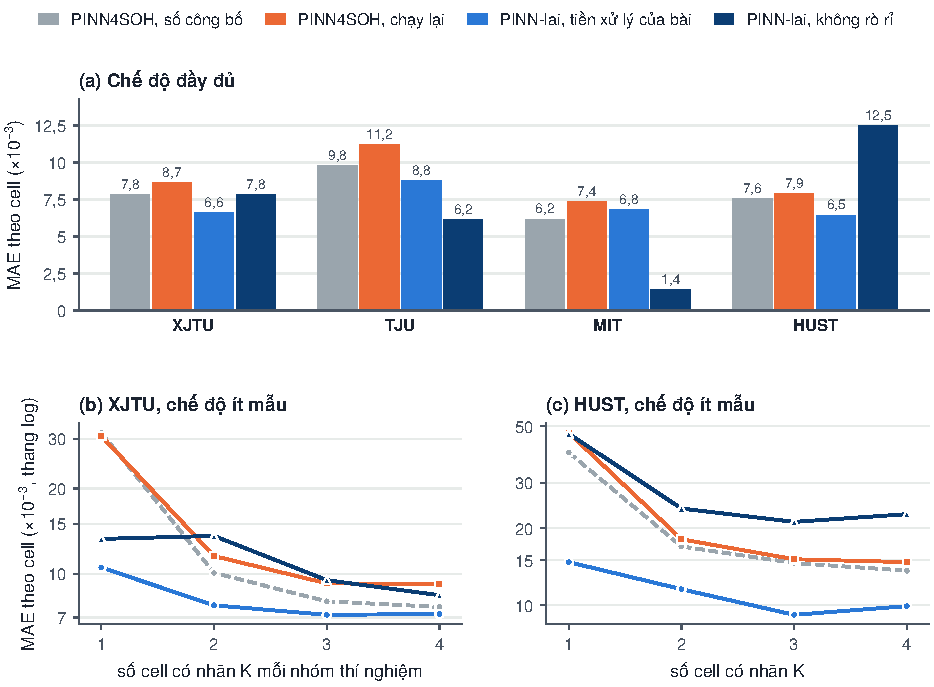
\includegraphics[width=\textwidth]{graphics/fig_benchmark.pdf}
\caption[So với PINN4SOH trên đúng cách chia của bài]{MAE theo cell trên đúng các nhóm đánh giá của bài PINN4SOH. (a) Chế độ đầy đủ, mỗi bộ bốn cột: số công bố của bài, mã gốc của bài chạy lại, PINN-lai với tiền xử lý của bài và PINN-lai với tiền xử lý không rò rỉ. (b), (c) Chế độ ít mẫu: MAE theo số cell có nhãn $K$.}\label{fig:bench}
\end{figure}

Theo RMSE, Bảng~\ref{tab:pubrmse} lấy trên mỗi bộ mô hình có sai số thấp nhất của đồ án và ghi tên mô hình đó. RMSE thấp nhất của đồ án thấp hơn số công bố ở XJTU, TJU và HUST (XJTU: PINN-lai, 22{,}2\,\%; TJU: PINN-lai, 14{,}0\,\%; HUST: PINN-lai, 16{,}3\,\%). Ở MIT, GBDT cao hơn 0{,}2\,\%.

\begin{table}[!htbp]\centering\small
\caption[RMSE tốt nhất của đồ án so với PINN4SOH]{RMSE ($\times10^{-3}$) trên đúng cách chia của bài PINN4SOH, chế độ đầy đủ, cùng tiền xử lý với bài. Cột thứ hai tính từ tệp kết quả công bố cùng mã nguồn của bài; cột thứ ba là RMSE thấp nhất trong PINN-lai, GBDT và PINN-semi của đồ án, cột Mô hình ghi mô hình đạt được. Cả hai cột lấy trung bình qua cell kiểm tra, lần chạy và nhóm như Bảng~\ref{tab:pub}. In đậm: thấp hơn trong hai cột. Chênh lệch là RMSE của đồ án so với số công bố, âm là đồ án thấp hơn.}\label{tab:pubrmse}
\begin{tabular}{lrrlr}\toprule
Bộ dữ liệu & RMSE PINN4SOH công bố $\downarrow$ & RMSE tốt nhất của đồ án $\downarrow$ & Mô hình & Chênh lệch $\downarrow$ \\\midrule
XJTU & 10{,}88 & \textbf{8{,}47} & PINN-lai & $-$22{,}2\,\% \\
TJU & 12{,}28 & \textbf{10{,}56} & PINN-lai & $-$14{,}0\,\% \\
MIT & \textbf{7{,}51} & 7{,}52 & GBDT & $+$0{,}2\,\% \\
HUST & 8{,}69 & \textbf{7{,}27} & PINN-lai & $-$16{,}3\,\% \\
\bottomrule\end{tabular}\end{table}

\subsection{Các chỉ số tốt hơn các bài báo đã công bố}
Cùng cách chia và cùng tiền xử lý với bài, PINN-lai có sai số thấp hơn mã gốc PINN4SOH chạy lại ở 12 trên 12 chế độ, thấp hơn có ý nghĩa thống kê ở 7 (tỉ số 0{,}76--0{,}92 ở chế độ đầy đủ, 0{,}31--0{,}79 ở chế độ ít mẫu) và không chế độ nào cao hơn có ý nghĩa thống kê (Bảng~\ref{tab:pub}). So với số công bố của PINN4SOH, PINN-lai thấp hơn ở 11 trên 12 chế độ (tỉ số 0{,}84--1{,}10 ở chế độ đầy đủ, 0{,}33--0{,}94 ở chế độ ít mẫu). Lợi thế lớn nhất ở chế độ ít mẫu, nơi hàm mất mát vật lý được tính cả trên các cell huấn luyện không nhãn. So với MLP và CNN mà bài PINN4SOH báo cáo, PINN-lai thấp hơn MLP ở 12 trên 12 chế độ và thấp hơn CNN ở 11 trên 12. Với tiền xử lý không rò rỉ, PINN-lai vẫn thấp hơn số công bố của PINN4SOH trên TJU (tỉ số 0{,}63), MIT (tỉ số 0{,}23), thấp hơn có ý nghĩa thống kê theo cell ở 2 trên 4 bộ đầy đủ, và ở XJTU $K = 1$ (tỉ số 0{,}42).

\subsection{Các chỉ số chưa tốt}
So với các bài báo đã công bố, đồ án còn một số điểm chưa đạt. Cùng điều kiện với bài, PINN-lai chưa thấp hơn số công bố của PINN4SOH ở MIT đầy đủ (6{,}80 so với 6{,}18), và chưa thấp hơn CNN của bài ở MIT đầy đủ (6{,}15). Một GBDT đơn giản với cùng tiền xử lý rò rỉ tốt ngang PINN-lai: tỉ số GBDT/PINN-lai 0{,}69--1{,}06, GBDT thấp hơn có ý nghĩa thống kê ở 2 chế độ (HUST $K = 1$, HUST $K = 2$) và không chế độ nào cao hơn. Với min--max theo cell, chỉ số chu kỳ đã chuẩn hoá là phần đời đã qua và mô hình cây khai thác thẳng thông tin này, nên lợi thế so với mã gốc trong điều kiện đó không thể quy cho phần vật lý. Với tiền xử lý không rò rỉ, PINN-lai cao hơn số công bố trên HUST (tỉ số 1{,}65), ngang trên XJTU (0{,}99), cao hơn có ý nghĩa thống kê theo cell ở 1 trên 4 bộ đầy đủ. Ở chế độ ít mẫu cao hơn ở 7 trên 8 (tỉ số 1{,}10--1{,}66). Đây là các chế độ mà tiền xử lý của bài có lợi nhiều nhất: khi chỉ có vài cell có nhãn, biết cell đã đi được bao nhiêu phần đời gần như là biết SOH. Đồ án không dùng tiền xử lý đó vì nó không thực hiện được khi triển khai (Mục~\ref{sec:dt_bo}). Đồ án không tái lập được chính xác số công bố của PINN4SOH: mã gốc chạy lại cho sai số bằng 1{,}04--1{,}19 lần ở chế độ đầy đủ, cao hơn có ý nghĩa thống kê theo cell ở 2 trên 4 bộ (Bảng~\ref{tab:pub}). Các hàng huấn luyện dựng lại trùng với dữ liệu của bài, nên phần chênh đến từ phần cứng và phiên bản thư viện.

Ngay trong các so sánh của chính đồ án, một số chỉ số cũng chưa đạt. GBDT đơn lẻ có sai số thấp hơn PINN-semi ở 14/16 trường hợp bộ $\times$ mức nhãn (10 có ý nghĩa thống kê). PINN-semi chỉ vượt GBDT có ý nghĩa thống kê ở HUST 30\,\% nhãn (Mục~\ref{sec:labels}). PINN-lai cố định vẫn kém GBDT có ý nghĩa thống kê ở TJU 70\,\%. Ở 70\,\% nhãn, PINN-semi kém MLP có ý nghĩa thống kê trên TJU (tỉ số 1{,}09). Với kiểm định bảo thủ ở mức fold, lợi ích ở 30\,\% nhãn chỉ đứng vững trên MIT. Khoảng dự đoán 90\,\% của ước lượng SOH có độ phủ thực tế 84{,}9--92{,}6\,\% (trung bình 88{,}8\,\%), 14--25\,\% số cell có độ phủ dưới 80\,\%. Với HiPINN (\Cref{sec:e33res}), khoảng SOH 90\,\% tính bằng phương pháp conformal phủ 89--93\,\% tuỳ bộ và ngân sách, khoảng RUL 90\,\% phủ 68--87\,\%. Tỉ lệ dự báo RUL nằm trong $\pm 20\,\%$ RUL thật là 53--84\,\%. Ở 10\,\% đời cuối của XJTU, MAE của HiPINN vẫn là 30{,}0 ($\times10^{-3}$). Tham số vật lý $\lambda$, $E_a$ không được dữ liệu xác định, và tốc độ $r$ học được thấp hơn nhiều tốc độ suy giảm thực đo (\Cref{sec:vatly}). Bộ lọc xu thế không bảo đảm SOH dự đoán không tăng (đầu ra tăng ở 28--44\,\% số bước). Ép không tăng làm sai số trên XJTU tăng 1{,}76--1{,}94 lần vì dung lượng đo được của XJTU tăng ở đầu đời.

\subsection{Vai trò của phần vật lý}\label{sec:vatly}
Đề tài nhấn mạnh sự hỗ trợ của thông tin hoá lý, nên cần nói rõ phần vật lý trong PINN-semi thực sự đóng góp gì. Ba quan sát ở các mục trước cho thấy đóng góp này hẹp hơn tên gọi. Thứ nhất, chỉ riêng ràng buộc đơn điệu đã mang lại 62--95\,\% mức giảm sai số của PINN-semi so với MLP ở 30\,\% nhãn, còn bỏ phần dư động học và ràng buộc miền chỉ làm MAE tăng 1--11\,\% (\Cref{sec:source}). Thứ hai, các tham số hoá lý dịch chuyển ít so với giá trị khởi tạo: $\lambda$ (khởi tạo bằng 1) của các PINN-semi nằm trong khoảng 0{,}96--0{,}98 ở XJTU, 0{,}95--0{,}97 ở TJU, 0{,}95--0{,}97 ở MIT và 0{,}90--1{,}26 ở HUST, còn $E_a$ khởi tạo ở 30\,kJ/mol thì dịch không quá 1{,}6\,kJ/mol. Thứ ba, tốc độ $r$ học được trung bình chỉ 0{,}001--0{,}063, trong khi tốc độ suy giảm thực đo là 0{,}137--0{,}356 SOH trên 1\,000 chu kỳ. Cả ba có nguyên nhân trong cách đặt bài toán, không phải do tối ưu chưa hội tụ.

Phần dư động học ràng buộc đạo hàm riêng $\partial u/\partial t$ khi giữ nguyên đặc trưng sạc. Trên quỹ đạo thật của một cell, SOH thay đổi chủ yếu vì đặc trưng sạc thay đổi theo tuổi, tức qua số hạng $\nabla_{\mathbf{x}} u \cdot \mathrm{d}\mathbf{x}/\mathrm{d}n$, còn $t$ chỉ là một trong 17 đầu vào. Mạng nghiệm vì vậy thoả được phương trình với một đạo hàm riêng nhỏ theo $t$, và $r$ học được nhỏ hơn nhiều so với tốc độ suy giảm thật. Với trọng số $\alpha = 0{,}02$, phần dư này chủ yếu buộc đạo hàm theo $t$ không dương, điều mà ràng buộc đơn điệu đã làm trực tiếp hơn.

Hệ số $\lambda$ khó xác định vì thừa số $g(u) = e^{\lambda(1-u)}$ chỉ thay đổi khoảng 22\,\% khi SOH đi từ 1 xuống 0,8 với $\lambda \approx 1$. Sự phụ thuộc vào mức suy giảm này đã có sẵn trong $k(\tilde{\mathbf{x}})$, vốn nhận các đặc trưng sạc biến thiên theo tuổi. Hai thừa số thay thế được cho nhau, nên dữ liệu chỉ kéo $\lambda$ đi một đoạn ngắn khỏi giá trị khởi tạo, xa nhất ở HUST.

Năng lượng hoạt hoá $E_a$ thì không định danh được về mặt toán học trên ba bộ. Thừa số Arrhenius $A(T) = \exp[-(E_a/R_g)(1/T - 1/T_\text{ref})]$ chỉ khác 1 khi nhiệt độ khác $T_\text{ref}$. Ở XJTU, mọi cell chạy ở 298{,}15\,K, đúng bằng $T_\text{ref}$, nên $1/T - 1/T_\text{ref} = 0$, $A \equiv 1$ và gradient của hàm mất mát theo $E_a$ bằng 0. Thực tế $E_a$ của mọi PINN-semi trên XJTU giữ đúng 30{,}0\,kJ/mol. Ở MIT và HUST, nhiệt độ là hằng 303{,}15\,K, nên $A$ chỉ là một hằng số nhân và bị $k(\tilde{\mathbf{x}}) = \operatorname{softplus}(G_\theta(\tilde{\mathbf{x}}))$ hấp thụ: mọi giá trị $E_a$ cho cùng một $r$ nếu $G_\theta$ bù lại. Chỉ TJU có ba mức nhiệt độ (298{,}15, 308{,}15 và 318{,}15\,K), nơi $E_a$ về nguyên tắc định danh được. Nhưng ở đó nhiệt độ chỉ làm sai số thay đổi dưới 1\,\% (thêm $1/T$ vào GBDT cho tỉ số 0{,}99--1{,}00, \Cref{sec:dt_bo}), nên dữ liệu cũng không đủ để ước lượng $E_a$ chính xác.

Dù vậy, phần vật lý vẫn có giá trị ở ba điểm. Một là ràng buộc đơn điệu và ràng buộc miền là tiên nghiệm vật lý đúng, và chúng được áp lên cả cell không nhãn. Ở 10\,\% nhãn, phần lợi ích do áp hàm mất mát vật lý lên cell không nhãn (PINN-semi so với PINN-sup, tỉ số 0{,}62--0{,}94) chiếm 50--64\,\% mức giảm sai số so với MLP. Hai là dạng tốc độ có cấu trúc, luôn không âm, ngăn lời giải tầm thường $G \approx u_t$ của động học hộp đen kiểu PINN4SOH, nên các ràng buộc thực sự tác động lên mạng nghiệm. Ba là ở bài toán dự báo, nghiệm đóng của cùng động học xám cho PINN-dự báo một đường ngoại suy có dạng vật lý: luôn không tăng, có thể gãy dần hoặc chậm dần, với chỉ hai tham số. PINN-dự báo là một trong ba nhánh của HiPINN. Vì vậy cụm “thông tin hoá lý” trong đồ án nên được hiểu là các tiên nghiệm có cấu trúc (đơn điệu, miền giá trị, tốc độ không âm, dạng Arrhenius, dạng nghiệm đóng), chứ không phải việc xác định các tham số điện hoá của cell.

\subsection{Nhận xét}
Trên đúng cách chia của PINN4SOH và cùng cách tính sai số, PINN-lai của đồ án có sai số thấp hơn số công bố ở phần lớn các chế độ và thấp hơn mã gốc chạy lại ở mọi chế độ. Tuy vậy, trong điều kiện có rò rỉ của bài, một GBDT cũng đạt kết quả tương tự, còn khi bỏ rò rỉ thì hơn hay kém tuỳ bộ dữ liệu. Vì thế, những đóng góp có cơ sở vững nhất của đồ án là giao thức đánh giá không rò rỉ, các so sánh ghép cặp có kiểm định trong cùng một giao thức, và các mô hình có đặc trưng lịch sử HiGBDT, HiPINN cho bài toán dự báo.


%% ============================================================================ CHƯƠNG 7
\chapter{Kết luận}\label{ch:ketluan}

\section{Những việc đã làm được}

\begin{enumerate}
\item Xây dựng đường ống dữ liệu cho bốn bộ dữ liệu công khai (387 cell, 305.802 chu kỳ sau lọc) với bộ lọc ngoại lai nhân quả, và kiểm tra bằng số liệu vì sao dùng 16 đặc trưng sạc cùng chỉ số chu kỳ, vì sao bỏ các cách biến đổi khác (Mục~\ref{ch:dactrung}).
\item Thiết kế giao thức đánh giá không rò rỉ và đo tác động của các dạng rò rỉ: chia theo chu kỳ làm sai số thấp đi 1{,}2--1{,}8 lần, chuẩn hoá theo cả vòng đời cell làm sai số đổi 0{,}46--2{,}76 lần tuỳ bộ.
\item Đề xuất PINN bán giám sát với động học xám luôn không âm: ở 10\,\% nhãn sai số bằng 0{,}39--0{,}90 lần MLP, tiết kiệm 1{,}7--4{,}5 lần số nhãn; và mô hình kết hợp PINN-lai: 0{,}67--0{,}95 lần PINN-semi, thấp hơn GBDT ở 10/16 trường hợp.
\item So sánh có kiểm định với chín mô hình đối chứng, gồm bốn mô hình học sâu của đề cương (MLP, CNN, LSTM, Transformer), bằng MAE, RMSE, MAPE và $R^2$.
\item Chạy lại mã gốc PINN4SOH trên đúng 39 nhóm của bài (390 lần chạy bản công bố, 117 lần bản đã sửa), phát hiện loss đơn điệu của bản đã sinh số công bố không có gradient, và so cùng điều kiện: PINN-lai thấp hơn mã gốc chạy lại ở 12/12 chế độ, thấp hơn số công bố ở 11/12.
\item Đặt lại bài toán ít nhãn theo số lần đo dung lượng: đo thưa mọi cell với 1{,}2--6{,}0\,\% số chu kỳ cho sai số bằng 0{,}85--0{,}93 lần gắn nhãn đầy đủ cho 30\,\% số cell; mở rộng sang dự báo SOH, dung lượng còn lại và RUL.
\item Kết hợp GBDT có đặc trưng lịch sử SOH (mã của repo G-doan) với PINN-dự báo, đánh giá trong một giao thức đã sửa các điểm còn rò rỉ của E22 (E33, \Cref{sec:e33res}): khi có lịch sử đo dung lượng, GBDT lịch sử có MAE bằng 0{,}85--0{,}94 lần GBDT theo tầm, mô hình kết hợp mới bằng 0{,}79--0{,}99 lần kết hợp E22 và 1{,}01--1{,}48 lần GBDT lịch sử; với lịch sử ước lượng, kết hợp mới bằng 0{,}90--1{,}01 lần kết hợp E22. Theo quy tắc chọn sau thí nghiệm, với SOH, không mô hình nào thoả ở cả ba thiết lập, vì GBDT lịch sử có MAE trung bình thấp hơn từng mô hình còn lại trên ít nhất ba bộ nhưng kém có ý nghĩa trên TJU so với kết hợp mới và kết hợp E22; khi có lịch sử đo, GBDT lịch sử có MAE trung bình thấp nhất trên cả bốn bộ ở cả hai ngân sách; với RUL, quy tắc chọn kết hợp E22 ở cả hai kịch bản lịch sử.
\item Tổ chức lại mã nguồn thành các khối dữ liệu, mô hình, thí nghiệm, phân tích, so sánh với PINN4SOH, bản thảo bài báo và báo cáo; 11.429 lượt huấn luyện có kết quả trong báo cáo, mọi bảng sinh tự động từ kết quả, chạy lại cho kết quả trùng từng bit (Mục~\ref{sec:tailap}).
\end{enumerate}


\section{Những việc chưa làm được}

\begin{enumerate}
\item Một mô hình cây đơn giản (GBDT) vẫn là đối thủ khó nhất: PINN-semi đơn lẻ chưa vượt được nó khi có từ 30\,\% nhãn,
      và chỉ khi ghép với GBDT (PINN-lai) mới thấp hơn ở phần lớn trường hợp. Ràng buộc vật lý chưa được đưa vào chính mô
      hình cây.
\item Không tái lập được chính xác số công bố của PINN4SOH vì không dựng lại được môi trường gốc (GPU, phiên bản thư viện);
      đồ án báo cáo cả số công bố lẫn số chạy lại.
\item Khoảng dự đoán 90\,\% chưa đạt độ phủ danh nghĩa; tham số vật lý $\lambda, E_a$ không được dữ liệu xác định; tốc độ
      $r$ của dạng đạo hàm riêng không phải tốc độ suy giảm thật của cell.
\item Các phân tích hậu kiểm (tinh chỉnh trọng số ghép, chọn có hay không lịch sử) chưa được kiểm chứng trên dữ liệu mới;
      PINN-lai và các thí nghiệm về sau dùng 3 thay vì 5 lần lặp.
\item Chưa xử lý dữ liệu thô của từng bộ, nên chưa thử được các đặc trưng cần đường cong đầy đủ; chưa có dữ liệu vận
      hành ngoài phòng thí nghiệm và dữ liệu nhiều cell ghép song song (giai đoạn 2 của đề cương).
\end{enumerate}

\begin{thebibliography}{99}\small\setlength{\itemsep}{0pt}\setlength{\parsep}{0pt}
\bibitem{angelopoulos2023} A. N. Angelopoulos, S. Bates. Conformal prediction: a gentle introduction.
  \emph{Foundations and Trends in Machine Learning}, 16(4):494--591, 2023.
\bibitem{arlot2010} S. Arlot, A. Celisse. A survey of cross-validation procedures for model selection.
  \emph{Statistics Surveys}, 4:40--79, 2010.
\bibitem{attia2022knee} P. M. Attia, A. Bills, F. Brosa Planella, et al. Review---``Knees'' in lithium-ion battery
  aging trajectories. \emph{Journal of The Electrochemical Society}, 169:060517, 2022.
\bibitem{bai2018tcn} S. Bai, J. Z. Kolter, V. Koltun. An empirical evaluation of generic convolutional and recurrent
  networks for sequence modeling. arXiv:1803.01271, 2018.
\bibitem{birkl2017} C. R. Birkl, M. R. Roberts, E. McTurk, P. G. Bruce, D. A. Howey. Degradation diagnostics for
  lithium ion cells. \emph{Journal of Power Sources}, 341:373--386, 2017.
\bibitem{bouckaert2004} R. R. Bouckaert, E. Frank. Evaluating the replicability of significance tests for comparing
  learning algorithms. \emph{Advances in Knowledge Discovery and Data Mining (PAKDD)}, 3--12, 2004.
\bibitem{breiman1996} L. Breiman. Bagging predictors. \emph{Machine Learning}, 24(2):123--140, 1996.
\bibitem{breiman2001rf} L. Breiman. Random forests. \emph{Machine Learning}, 45(1):5--32, 2001.
\bibitem{broussely2001} M. Broussely, S. Herreyre, P. Biensan, et al. Aging mechanism in Li ion cells and calendar
  life predictions. \emph{Journal of Power Sources}, 97--98:13--21, 2001.
\bibitem{cleveland1979} W. S. Cleveland. Robust locally weighted regression and smoothing scatterplots.
  \emph{Journal of the American Statistical Association}, 74(368):829--836, 1979.
\bibitem{dietterich1998} T. G. Dietterich. Approximate statistical tests for comparing supervised classification
  learning algorithms. \emph{Neural Computation}, 10(7):1895--1923, 1998.
\bibitem{efron1993} B. Efron, R. J. Tibshirani. \emph{An Introduction to the Bootstrap}. Chapman \& Hall, 1993.
\bibitem{fermin2020} P. Fermín-Cueto, E. McTurk, M. Allerhand, et al. Identification and machine learning
  prediction of knee-point and knee-onset in capacity degradation curves of lithium-ion cells. \emph{Energy and AI},
  1:100006, 2020.
\bibitem{friedman2001} J. H. Friedman. Greedy function approximation: a gradient boosting machine.
  \emph{Annals of Statistics}, 29(5):1189--1232, 2001.
\bibitem{grinsztajn2022} L. Grinsztajn, E. Oyallon, G. Varoquaux. Why do tree-based models still outperform deep
  learning on typical tabular data? \emph{Advances in Neural Information Processing Systems}, 35, 2022.
\bibitem{guyon2003} I. Guyon, A. Elisseeff. An introduction to variable and feature selection. \emph{Journal of
  Machine Learning Research}, 3:1157--1182, 2003.
\bibitem{he2011} W. He, N. Williard, M. Osterman, M. Pecht. Prognostics of lithium-ion batteries based on
  Dempster--Shafer theory and the Bayesian Monte Carlo method. \emph{Journal of Power Sources}, 196(23):10314--10321,
  2011.
\bibitem{hinton2015} G. Hinton, O. Vinyals, J. Dean. Distilling the knowledge in a neural network.
  arXiv:1503.02531, 2015.
\bibitem{hochreiter1997} S. Hochreiter, J. Schmidhuber. Long short-term memory. \emph{Neural Computation},
  9(8):1735--1780, 1997.
\bibitem{holm1979} S. Holm. A simple sequentially rejective multiple test procedure. \emph{Scandinavian Journal of
  Statistics}, 6(2):65--70, 1979.
\bibitem{hu2020joule} X. Hu, L. Xu, X. Lin, M. Pecht. Battery lifetime prognostics. \emph{Joule}, 4(2):310--346,
  2020.
\bibitem{kapoor2023} S. Kapoor, A. Narayanan. Leakage and the reproducibility crisis in machine-learning-based
  science. \emph{Patterns}, 4(9):100804, 2023.
\bibitem{karniadakis2021} G. E. Karniadakis, I. G. Kevrekidis, L. Lu, P. Perdikaris, S. Wang, L. Yang.
  Physics-informed machine learning. \emph{Nature Reviews Physics}, 3:422--440, 2021.
\bibitem{ke2017} G. Ke, Q. Meng, T. Finley, et al. LightGBM: a highly efficient gradient boosting decision tree.
  \emph{Advances in Neural Information Processing Systems}, 30, 2017.
\bibitem{kohavi1997} R. Kohavi, G. H. John. Wrappers for feature subset selection. \emph{Artificial Intelligence},
  97(1--2):273--324, 1997.
\bibitem{krishnapriyan2021} A. S. Krishnapriyan, A. Gholami, S. Zhe, R. M. Kirby, M. W. Mahoney. Characterizing
  possible failure modes in physics-informed neural networks. \emph{Advances in Neural Information Processing
  Systems}, 34, 2021.
\bibitem{lakshminarayanan2017} B. Lakshminarayanan, A. Pritzel, C. Blundell. Simple and scalable predictive
  uncertainty estimation using deep ensembles. \emph{Advances in Neural Information Processing Systems}, 30, 2017.
\bibitem{lee2013} D.-H. Lee. Pseudo-label: the simple and efficient semi-supervised learning method for deep neural
  networks. \emph{ICML Workshop on Challenges in Representation Learning}, 2013.
\bibitem{lei2018} J. Lei, M. G'Sell, A. Rinaldo, R. J. Tibshirani, L. Wasserman. Distribution-free predictive
  inference for regression. \emph{Journal of the American Statistical Association}, 113(523):1094--1111, 2018.
\bibitem{loshchilov2019} I. Loshchilov, F. Hutter. Decoupled weight decay regularization. \emph{International
  Conference on Learning Representations}, 2019.
\bibitem{ma2022} G. Ma, S. Xu, B. Jiang, et al. Real-time personalized health status prediction of lithium-ion
  batteries using deep transfer learning. \emph{Energy \& Environmental Science}, 15:4083--4094, 2022.
\bibitem{nadeau2003} C. Nadeau, Y. Bengio. Inference for the generalization error. \emph{Machine Learning},
  52:239--281, 2003.
\bibitem{pinson2013} M. B. Pinson, M. Z. Bazant. Theory of SEI formation in rechargeable batteries: capacity fade,
  accelerated aging and lifetime prediction. \emph{Journal of The Electrochemical Society}, 160(2):A243--A250, 2013.
\bibitem{raissi2019} M. Raissi, P. Perdikaris, G. E. Karniadakis. Physics-informed neural networks: a deep learning
  framework for solving forward and inverse problems involving nonlinear partial differential equations.
  \emph{Journal of Computational Physics}, 378:686--707, 2019.
\bibitem{rasmussen2006} C. E. Rasmussen, C. K. I. Williams. \emph{Gaussian Processes for Machine Learning}.
  MIT Press, 2006.
\bibitem{saxena2008} A. Saxena, J. Celaya, E. Balaban, et al. Metrics for evaluating performance of prognostic
  techniques. In \emph{International Conference on Prognostics and Health Management}, IEEE, 2008.
\bibitem{schmalstieg2014} J. Schmalstieg, S. Käbitz, M. Ecker, D. U. Sauer. A holistic aging model for
  Li(NiMnCo)O$_2$ based 18650 lithium-ion batteries. \emph{Journal of Power Sources}, 257:325--334, 2014.
\bibitem{severson2019} K. A. Severson, P. M. Attia, N. Jin, et al. Data-driven prediction of battery cycle life before
  capacity degradation. \emph{Nature Energy}, 4:383--391, 2019.
\bibitem{strobl2008} C. Strobl, A.-L. Boulesteix, T. Kneib, T. Augustin, A. Zeileis. Conditional variable importance
  for random forests. \emph{BMC Bioinformatics}, 9:307, 2008.
\bibitem{tarvainen2017} A. Tarvainen, H. Valpola. Mean teachers are better role models: weight-averaged consistency
  targets improve semi-supervised deep learning results. \emph{Advances in Neural Information Processing Systems},
  30, 2017.
\bibitem{thelen2024} A. Thelen, X. Huan, N. Paulson, S. Onori, Z. Hu, C. Hu. Probabilistic machine learning for
  battery health diagnostics and prognostics---review and perspectives. \emph{npj Materials Sustainability}, 2:14,
  2024.
\bibitem{varma2006} S. Varma, R. Simon. Bias in error estimation when using cross-validation for model selection.
  \emph{BMC Bioinformatics}, 7:91, 2006.
\bibitem{vaswani2017} A. Vaswani, N. Shazeer, N. Parmar, et al. Attention is all you need. \emph{Advances in Neural
  Information Processing Systems}, 30, 2017.
\bibitem{vovk2005} V. Vovk, A. Gammerman, G. Shafer. \emph{Algorithmic Learning in a Random World}. Springer, 2005.
\bibitem{waldmann2014} T. Waldmann, M. Wilka, M. Kasper, M. Fleischhammer, M. Wohlfahrt-Mehrens. Temperature
  dependent ageing mechanisms in lithium-ion batteries -- a post-mortem study. \emph{Journal of Power Sources},
  262:129--135, 2014.
\bibitem{wang2011lfp} J. Wang, P. Liu, J. Hicks-Garner, et al. Cycle-life model for graphite-LiFePO$_4$ cells.
  \emph{Journal of Power Sources}, 196(8):3942--3948, 2011.
\bibitem{wang2021grad} S. Wang, Y. Teng, P. Perdikaris. Understanding and mitigating gradient flow pathologies in
  physics-informed neural networks. \emph{SIAM Journal on Scientific Computing}, 43(5):A3055--A3081, 2021.
\bibitem{wang2024} F. Wang, Z. Zhai, Z. Zhao, Y. Di, X. Chen. Physics-informed neural network for lithium-ion
  battery degradation stable modeling and prognosis. \emph{Nature Communications}, 15:4332, 2024.
\bibitem{wilcoxon1945} F. Wilcoxon. Individual comparisons by ranking methods. \emph{Biometrics Bulletin},
  1(6):80--83, 1945.
\bibitem{wolpert1992} D. H. Wolpert. Stacked generalization. \emph{Neural Networks}, 5(2):241--259, 1992.
\bibitem{zhang2018lstm} Y. Zhang, R. Xiong, H. He, M. G. Pecht. Long short-term memory recurrent neural network for
  remaining useful life prediction of lithium-ion batteries. \emph{IEEE Transactions on Vehicular Technology},
  67(7):5695--5705, 2018.
\bibitem{zhu2022} J. Zhu, Y. Wang, Y. Huang, et al. Data-driven capacity estimation of commercial lithium-ion
  batteries from voltage relaxation. \emph{Nature Communications}, 13:2261, 2022.
\end{thebibliography}
\end{document}
